\chapter*{Synopsis}
\addcontentsline{toc}{chapter}{Synopsis} 
\renewcommand{\figurename}{Figure}
\renewcommand{\thefigure}{\arabic{figure}} % Plain numbering
\setcounter{figure}{0}                     % Reset if needed

\begin{center}
    General thesis summary
\end{center}

\section*{Relevance}
Quantum key distribution (QKD) is a relevant technology emerging from quantum information science theory that allows a symmetric bit sequence to be distributed using quantum techniques to two or more users to use this sequence as a key for symmetric data encryption while simultaneously detecting unauthorized access by illegitimate users. The use of quantum states of light in the key distribution allows to achieve a level of secrecy unavailable to classical encryption protocols. Such quantum states can be represented as single photons. Their quantum properties do not allow an attacker to copy their states or read them without modification and without introducing errors. Such quantum states can be transmitted both through fiber-optic communication lines (FOCL), atmospheric channels and in outer space by means of satellites. The principle of operation of these systems is as follows. On the transmitter side (Alice) quantum states are formed. For this purpose coherent laser radiation is used, attenuated to single photons with the help of attenuator. A change in the polarization or phase shift of the photon is introduced into the prepared quants of light. The state thus prepared is transmitted through a communication channel to the receiver (Bob). At the receiver side, the photon state is re-measured independently of Alice. In the case of Bob's correlation, the received single photon is detected by a single photon detector. Due to the properties of the single photon in the form of impossibility of cloning, impossibility of measurement without destruction and its indivisibility it is possible to trace the impact of the intruder, as his actions will lead to the appearance of errors in the received bit sequence. This is how the control of unauthorized access is ensured. 

A separate class are systems of quantum key distribution on continuous variables (CV-QKD). In such systems quantum state, prepared and transmitted by Alice, on the receiving side interacts with strong laser radiation. And the result of this interaction is registered by a balance detector. The main differences of this detector from the detector of single photons is the use of two classical photodetectors, connected in such a way that their photocurrents are mutually subtracted, which reduces the noise of the system, and the lack of cooling to temperatures of about -40$^{\circ}$ degrees Celsius. All of this allows for simplification of the final system. To the advantages of the FACS can be attributed a greater speed of secret key generation compared to the FAC systems on discrete variables, which use single photon detectors. 

Among the complexities of the CV-QKD systems is the method of transmission of strong laser radiation or local oscillator (LO) to the receiving side and its separation from the quantum signal. In the first Gaussian modulated CV-QKD systems, the Local Oscillator and quantum states were generated at the transmitter, combined and transmitted together in a quantum channel. At the receiving end, the local oscillator and the quantum signal are separated, the LO is delayed by a special delay line and reconnected at the beam splitter for interaction. The result of this interaction is an interference pattern whose intensity distribution depends on the state encoded by Alice. The resulting field is registered by a balance detector, at the output of which a voltage level is formed, which is further subjected to post-processing.  Transmission of the local oscillator through the channel limits the range of operation of this type of system and limits the speed of key generation, because for the best operation of the system requires LO as much power as possible. The second problem is the ability of an attacker to manipulate the local oscillator to create information leakage channels. As an alternative, it is proposed to use a local oscillator generated at the receiving side. Such a solution will increase the range of key transmission, the speed of its generation and close the vulnerability to an attack on LO.
One of the promising approaches to the realization of quantum communication systems on continuous variables is the system of quantum communication on side frequencies of modulated radiation. The basis of this method is the transfer of the quantum channel to side frequencies, which appear as a result of modulation of optical radiation by an alternating electric field. This increases the stability of the transmitted signal to external influences and provides a high spectral efficiency, as well as provides indicators for the ratio of the rate of key generation to the distance between the receiver and transmitter units, comparable to other systems of quantum communication. This method is also suitable for realizing continuous variable protocols with coherent detection methods. In particular, this paper considers a heterodyne method in which the quantum states prepared by Alice are transmitted over a fiber link to the receiver, in it they fall on a 2x2 beam splitter with a 50:50 splitting ratio and are mixed on it with a powerful local oscillator, which is detuned in frequency from the transmitting laser by an amount that exceeds the frequency of the state change. The result of the interference is detected by a balance detector. The output of the balance detector produces a signal at an intermediate frequency from the entire spectrum of the signal transmitted by Alice. Extraction of information requires filtering using low pass filter and demodulation of the received signal to generate a raw key. 

One of the challenges in implementing heterodyne detection method for key distribution is the need to compensate for phase noise. Various methods are used for this purpose. The first of these methods is the transmission of a 'pilot tone', during detection of which the phase noise contributed by the channel is measured. The measured value is then taken into account in the post-processing of the states. The second is the implementation of feedback in various forms. Within the scope of this paper, an optical feedback method is proposed for a quantum key distribution system at side frequencies on continuous variables. The essence of this method is the injection of laser radiation from the master laser, which is the transmitter laser, into the slave laser, which is used as a local oscillator in the receiver. This method allows stabilizing the LO wavelength and reducing phase noise due to the fact that both sources are coherent radiation generators with random phase.
The optical injection method requires an additional channel to transmit the feedback generation. Such a channel increases system complexity and fiber optic link (FOCL) requirements, which is particularly critical in urban links where the allocation of an additional fiber or channel in multiplexed networks is difficult. The solution to this problem may be a system of quantum key distribution on continuous variables using heterodyne detection with independent LO. The essence of this system is that the receiver and transmitter are equipped with wavelength stabilized lasers with a spectral line width of less than 10 kHz. This approach allows to avoid constant adjustment of the laser wavelengths and to reduce the phase noise associated with the independence of the radiation sources.
However, the phase noise does not disappear, so it still needs to be compensated. In the case of implementing such a signal detection method for a quantum key distribution protocol at side frequencies, the carrier frequency can be used for this purpose by measuring its phase and making adjustments in post-processing. 

The differences between real QKD systems and the models used for theoretical proofs can be exploited by an attacker to carry out different types of attacks on the equipment comprising the system. It has been shown in earlier works that laser radiation sources based on semiconductor crystals can be vulnerable to 'seeding' by an attacker's external radiation at a wavelength close to that used by the transmitter. This attack results in a change in the shape of the emitted pulse and an increase in output power, and in some cases a change in wavelength can also be observed. These effects result in an increase in the average number of photons emitted by the transmitter, which opens up the possibility of a photon number splitting attack for the attacker. 
However, 'seeding' attacks by laser radiation at other wavelengths have not been considered in the literature. This type of attack is more dangerous because passive fiber optic elements that introduce additional attenuation, such as isolators or DWDM filters, are used to protect against it. However, there are works that demonstrate that the amount of attenuation in such elements can be reduced when the incident wavelength of the radiation is significantly changed. For example, an insulator with an operating wavelength of 1550 nm introduces 50 dB of back-pass loss, when this value is 20 dB when exposed to radiation at a wavelength of 1310 nm. And in the case of the DWDM filter, it contributes virtually no attenuation at 1310 nm. Thus, it is much easier for an attacker to perform a 'seeding' attack with laser radiation, since the attenuation introduced at this wavelength is less. 

This type of attack is called an 'optical pumping attack'. Its essence is that the attacker probes the laser with a wavelength different from the operating wavelength. This radiation is absorbed by the active medium of the transmitter laser so that the absorbed radiation acts as an optical pump, which works as a complement to the electrical pump of the semiconductor laser. In this case, the Watt-Ampere characteristic of the laser and its quantum efficiency changes. This leads to the fact that the energy of the emitted pulses increases while the pump current remains unchanged. In the framework of this work, this type of attack is first labelled, the lower limit of the necessary radiation power at the wavelength of 1310 nm to change the characteristics of the laser under study is determined, and the effect of optical pumping on the laser characteristics is measured. 

In quantum distribution systems, laser radiation sources based on optical injection are used. Such sources are constructed in the following way: two lasers are used -- a master and a slave laser connected by a circulator. Radiation of the slave laser allows reducing the jitter of emitted pulses, stabilizing the output power and narrowing the spectral line. However, such sources have not been investigated for robustness to external radiation. Previously shown work on laser 'seeding' has been carried out only for single radiation sources. A source based on optical injection has several advantages relative to a single source: the presence of isolation from the quantum channel due to the optical circulator and the presence of external radiation from the leading laser. This work studies the effect of high-power laser radiation on the duration, jitter, and amplitude of the emitted pulses, and demonstrates a lower bound on the radiation power required to modify the operation of this system.

\section*{The goal}

To develop a system of heterodyne detection of signals in a quantum communication system at side frequencies with a local oscillator on the receiver side using optical injection and to investigate the resistance to attacks on the technical implementation of laser radiation sources in this system.
In order to achieve the goal in the framework of the thesis, the following objectives have been established:
\section*{Objectives}
\textbf{Objective 1: development of QKD system with feedback}\\
Implementation of optical injection feedback for sideband QKD system with heterodyne detection method and continuous variables\\

\textbf{Objective 2: research of heterodyne detectinon for SCW-QKD with two independent sources} \\
Application of heterodyne signal detection in QKD systems with two independent sources of laser radiaton and development of polartzation maitaining algorithm.\\

\textbf{Objective 3: experimental design}\\
Study the optical pumping attack on radiation sources that can be local oscillators for continuous variable quantum key distribution systems.\\

\textbf{Objective 4: research of influence of high power radiation to optical injection locked source.}\\
To investigate the effect of high-power optical radiation on a radiation source based on optical injection.
\section*{Research methods}
In the framework of this thesis, the following research methods were used\\
(an analysis of practical cases, an overview of the latest practices, etc.)

\section*{Assertions that are presented for defense}
\begin{enumerate}
    \item The use of optical injection method for the implementation of feedback in the system of quantum communication at side frequencies on continuous variables with discrete modulation and local oscillator implemented on the receiver side allows stabilising the wavelength of the radiation source on the transmitting side, which leads to the possibility of transmission of phase-encoded signals and their heterodyne reception through the fiber-optic channel.
    \item For quantum communications on the basis of coherent detection by heterodyne method of registration of multimode quantum states with phase coding on the basis of two independent sources of laser radiation with the use of frequency multiplexing on one carrier frequency and developed an algorithm to control the polarization of the incoming signal on the basis of fast Fourier transform method. 
    \item Seeding 1.6 mW of continuous mode optical power at 1310 nm into the resonator of a distributed feedback laser (Agilecom WSLS-934010C4124-82) with an operating wavelength of 1550 nm increases the average number of photons at 1550 nm by $21\%$, increases the output pulse energy by $10\%$, and increases the differential quantum efficiency of the attacked laser by $2\%$.
    \item Seeding 800 mW of intruder radiation continuously at 1549.7 nm into a slave laser (Agilecom WSLS-934010C4124-82) in an optical injection based source increases the standard deviation of the amplitude of the output pulses of the slave laser by $3\%$, increases the standard deviation of their energy by $3\%$, and increases the average radiated power by $8\%$.
\end{enumerate}


\section*{The novelty of research}
An optical injection feedback system for a quantum key distribution system at side frequencies is implemented for the first time and the sifted key is transmitted. A heterodyne signal detection method with two independent radiation sources is implemented for a quantum key distribution system at side frequencies and a polarization control algorithm is developed for this system. For the first time a new type of attack on the technical implementation - optical pumping attack on the radiation source in quantum key distribution systems, which allows to increase the emitted average number of photons bypassing the existing protection methods, is demonstrated. The influence of high-power laser radiation on the source of coherent radiation based on optical injection has been determined experimentally, which increases the energy of emitted pulses and its spread, increases the output power of the attacked source, which together leads to a decrease in the rate of secret key generation.

\section*{Theoretical and pratcical significance}

The theoretical significance of the work is determined by the fact that within the framework of it phase-encoded states in the system of quantum key distribution at side frequencies on continuous variables with heterodyne method of signal detection were transferred and the wavelengths of information laser and local oscillator laser were stabilized. Also within the framework of the work the exchange of phase-encoded states in the system of quantum distribution of keys at side frequencies on continuous variables with heterodyne method of signal detection and two independent sources of radiation of information signal and local oscillator was made, within the framework of transfer of such states the algorithm of adjustment of polarization of information radiation was worked out. The average output power and pulse energy of a distributed feedback laser used in quantum key distribution systems are increased by optical pumping at a wavelength of 1310 nm. The average output power and standard deviation of the amplitude of the output pulses emitted by a coherent radiation source based on optical injection with the help of high-power laser radiation of an intruder, leading to the creation of additional vulnerability on access to the secret key, is increased. 
Practical significance of the work lies in the fact that the conducted experimental studies on the implementation of heterodyne method of signal detection show the operability of this approach to create systems of quantum key distribution using this method of signal registration. Researched methods of the attacker's influence on the sources of radiation in the systems of quantum key distribution allows to improve the model of the intruder, increasing the resistance of the final systems of quantum key distribution to attacks on the technical implementation

\section*{Validity}
The reliability of the obtained results is based on the use of modern methods of scientific research and comparison of the obtained results with the data of scientific and technical literature. The approved methods and certified equipment were used in the research. Experimental data processing was carried out with the help of Origin and Python application software package. The materials were published in 9 printed papers and presented at 10 international and Russian conferences.

\section*{Implementation of research results}
(specify the degree of implementation; technologies, new universal measurement methods, educational technologies, etc.)

\section*{Approbation of research results}
Key research results were presented and discussed at the following conferences:
\begin{enumerate}
    \item CYS X 'Application of the heterodyne signal analysis method for implementing a quantum communication protocol with a star topology'
    \item IWQO-2021 'Application of the heterodyne signal analysis method for implementing a quantum communication protocol with a star topology'
    \item PPS LI 'Coherent reception in quantum communication systems at side frequencies with an untrusted receiving node'
    \item XI CYS 'Multi-user city-scale quantum networks based on passive optical networks'
    \item 20th International Conference Laser Optics ICLO 2022 'Continuous variable measurement-device-independent quantum communication scheme based on subcarrier waves'
    \item XII CYS 'Quantum communication system on continuous variables with an untrusted receiving node'
    \item LII scientific and educational-methodological conference of the teaching staff 'Frequency multiplexing for a quantum key distribution system on side frequencies'
    \item All-Russian scientific conference with international participation 'Nevskaya Photonics-2023' (09.10.2023 - 13.10.2023), 'Heterodyne detection for a quantum key distribution system at side frequencies with two independent radiation sources'
    \item 22nd International Conference Laser Optics ICLO 2024 'Laser-pumping attack on QKD sources', 1-5 July 2024
    \item 22nd International Conference Laser Optics ICLO 2024, 'Secure laser source for QKD systems', 1-5 July 2024
    \item QCrypt 2024, 2-6 September 2024, 'Optical pumping attack to laser source in Quantum key distribution system'
\end{enumerate}

Translated with DeepL.com (free version)
\section*{Personal contribution of the author}
(the author's participation in all the stages of research, such as data collection or execution of experiments, approbation of the obtained results, design of experimental panels and plants (key elements of experimental plants), processing and interpretation of experimental data, publication of research papers, etc.)

\section*{Thesis structure and number of pages}
\section*{Publications}
Key results of research are described in nine publications. Four of them are published in journals recommended by the Higher Attestation Commission and one is published in a journal indexed by Scopus. One certificate of state registration of a computer program has also been obtained.\\

Publications in international journals indexed by Scopus:\\
1.\\
2.\\
3.\\

Publications in journals from the list of the Russian Higher Attestation Commission:\\
1.\\
2.\\
3.\\

Publications in other journals:\\
1.\\
2.\\
3.

\section*{Основное содержание работы }
In the \underline{introduction} the relevance of the research conducted within the framework of the thesis work is justified, the purpose of the research is defined, the tasks of the work are set, the scientific novelty of the work, its theoretical and practical significance, as well as the possibility of implementation of its results are indicated. 
In the \newline In the \underline{first chapter} is given a review of the state of science and technology on the subject of quantum key distribution. Quantum communication protocols using both discrete\cite{bennett1984,bennett1992,ekert1991,wang2005b} and continuous variable\cite{yuan2005,andersen2010,dixon2010,hajomer2024,diamanti2015} are considered. The features of coherent detection methods\cite{ip2008a} used in quantum key distribution systems are described and analyzed. The issue of phase noise in quantum key distribution systems is highlighted. Examples of methods to compensate for phase noise are demonstrated, such as applying pilot pulses \cite{wang2020} and creating feedback \cite{khaksar2023a}.  Known attacker's attacks on equipment within QKD systems are shown \cite{lydersen2010a,gisin2006, huang2013}. The laser seeding attack on the transmitter laser, its impact and possible defense methods are described{\cite{huang2019,lovic2023,ma2013}. Another aspect under consideration is an attack on the power of the local oscillator transmitted in the channel for quantum key distribution systems on continuous variables, the principle of its implementation, the result of the attack and methods to counteract it\cite{jouguet2013,shao2022,fan2023,ren2019}.
\newline In the \underline{second chapter}, we investigate the optical injection method~\cite{shakhovoy2024,liu2020} for creating feedback in the quantum key distribution system at side frequencies\cite{gleim2016,gleim2017,fadeev2024}. The optical injection method is that there is a pair of lasers: a master laser and a slave laser. The radiation from the master laser is injected into the resonator of the slave laser. Injection of additional photons into the resonator of the slave laser reduces the relaxation oscillation time of the radiation, which accelerates the radiation generation process and reduces negative effects. This approach improves the emission characteristics of the slave laser in particular:
\begin{itemize}
    \item narrowing of the spectral line of the output radiation
    \item Reduction of nonlinearities and suppression of relaxation oscillations
    \item Reducing the output pulse chirp and increasing amplitude stability
\end{itemize}
This approach allows synchronizing the frequencies of the master and slave lasers, and as a consequence, reducing their relative phase noise, achieving phase synchronism. This effect allows optical injection to be used as a feedback implementation for the local oscillator in a QRC system at side frequencies using continuous variables. The result of the feedback application will be stabilization of the intermediate frequency and reduction of phase noise. To implement this method, a separate channel and circulator is used to separate the radiation of the master and slave laser. 
This method can be applied to a quantum key distribution system at side frequencies.
\begin{figure}
    \centering
    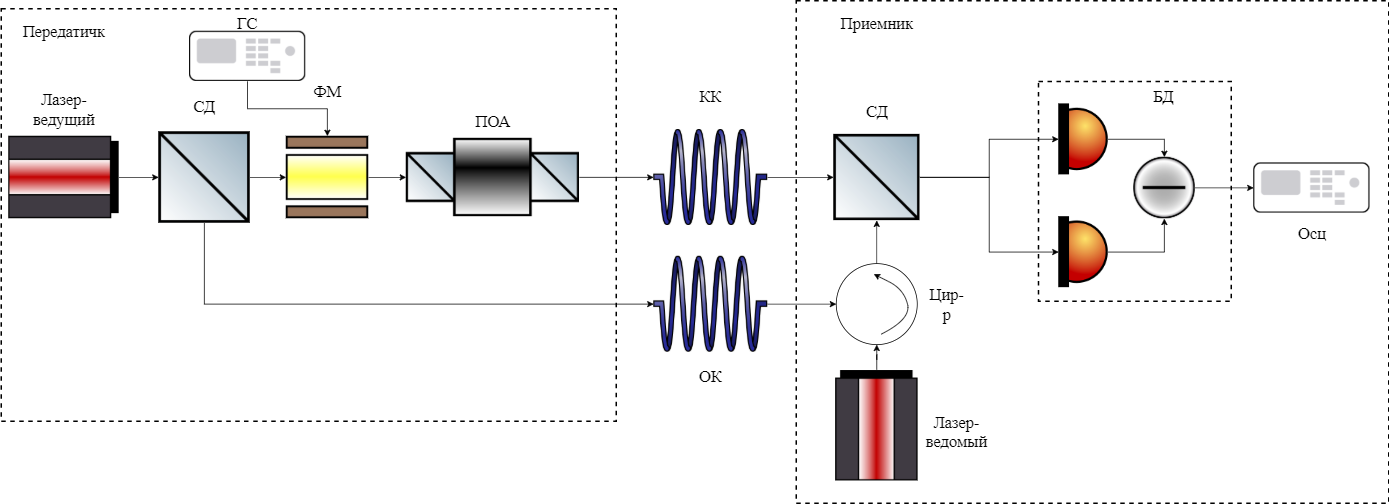
\includegraphics[width=\textwidth]{images/Схема с обратной связью.png}
    \caption{Schematic diagram of the QKD system experiment using optical injection. SD - beam splitter, FM - phase modulator, GS - signal generator, POA - tunable optical attenuator, QC - quantum channel, OC - open channel, Qir-r - circulator, BD - balance detector, Osz - oscilloscope}.
    \label{fig:opt inj scheme syn}
\end{figure}
This system, the optical scheme of which is shown in Figure~\ref{fig:opt inj scheme syn}, works as follows. At the transmitter side, the radiation generated by the laser is split into two parts. The first part of the radiation goes to an Alice phase modulator, where phase modulation by an alternating electrical signal takes place, in which phase shifts are introduced to encode the information. Quadrature Phase Shift Keying or Quadrature Phase Shift Keying (QPSK) modulation can be used as encoding. This digital modulation method introduces phase shifts corresponding to values of 45\textdegree, 135\textdegree, 225\textdegree and 315\textdegree. These phase shift values are assigned bit values {00, 01, 10, 11}. As a result, three harmonics of the signal appear in the spectrum: $\omega$ - the centre frequency of the laser, $\omega$ - $\Omega$ - the lower side frequency and $\omega$ + $\Omega$ - the upper side frequency, where $\Omega$ is the modulation frequency. The radiation after modulation is described by Eq:
\begin{align}
\label{eq:spectrum seed}
F_s(t) & = A_0 * \sin(\omega_0 t + \phi_0) + \frac{A_0 * m}{2} * (\sin((\omega_0 + \Omega)t + (\phi_0 + \phi (t))) - \notag \\\
&- \frac{A_0 * m}{2} * (\sin((\omega_0 - \Omega)t + (\phi_0 - \phi (t)))),
\end{align} where $A_0$ is the amplitude of the original radiation, $\omega$ is the centre frequency of the laser, $\omega$ - $\Omega$ is the lower side frequency and $\omega$ + $\Omega$ is the upper side frequency, $\Omega$ is the modulation frequency, $\phi_0$ is the phase of the original radiation, $\phi(t)$ is the phase of the modulating radiation, $t$ is the time, $m$ is the modulation index. Modulation index is the value of the ratio of power at side frequencies to the power in the whole spectrum. The modulation index is proportional to the amplitude of the modulating electrical signal.  The obtained spectrum falls on a variable optical attenuator, the attenuation of which is adjusted in such a way that at the side frequencies there is a power corresponding to a given average number of photons, when the carrier can remain classical. The prepared quantum states are transmitted into the quantum channel. 
The second part of the radiation passes through a separate fiber channel to the receiver side, where it enters the fiber circulator so that the radiation enters the slave laser resonator. 
The incoming radiation from the quantum channel enters the first input of a fiber beam splitter with two inputs and two outputs and a 50:50 splitting ratio. The second input of the beam splitter is a local oscillator, which is the radiation generated by a separate laser on the receiving side. Due to the presence of feedback in the form of optical injection, the wavelength of the laser on the receiving side is synchronized with the wavelength of the Alice laser. As a result, the LO and quantum states interfere at the beam splitter. As a result of this interference, additional harmonics at an intermediate frequency appear at the output of the beam splitter. These harmonics are $\omega$ - $f$ - the central frequency of the Alice laser minus the LO frequency, ($\omega$ - $\Omega$) - $f$ - the lower side frequency minus the LO frequency and ($\omega$ + $\Omega$) - $f$ - the upper side frequency minus the LO frequency, where $\Omega$ - the modulation frequency, $\omega$ - the Alice laser frequency, $f$ - the LO frequency. 
\newline The result of this interference is detected by a balance detector. This device is two classical photodiodes connected so that their currents are subtracted. This connection reduces the intrinsic noise of the detector. After that, the received current is passed to a low-pass filter to filter out the constant component. The resulting signal is amplified by an amplifier stage and sent to the ADC.  As a result, only one signal is formed at the output of the balance detector at the frequency coinciding with the modulation frequency on the transmitter side. The reason for this is that the wavelengths of the LO and the transmitter laser coincide due to feedback in the form of optical injection. Thus, only the ($\omega$ + $\Omega$) component $f$ remains at the detector output, and the rest is converted to a constant component, which is filtered out. 
\begin{figure}
    \centering
    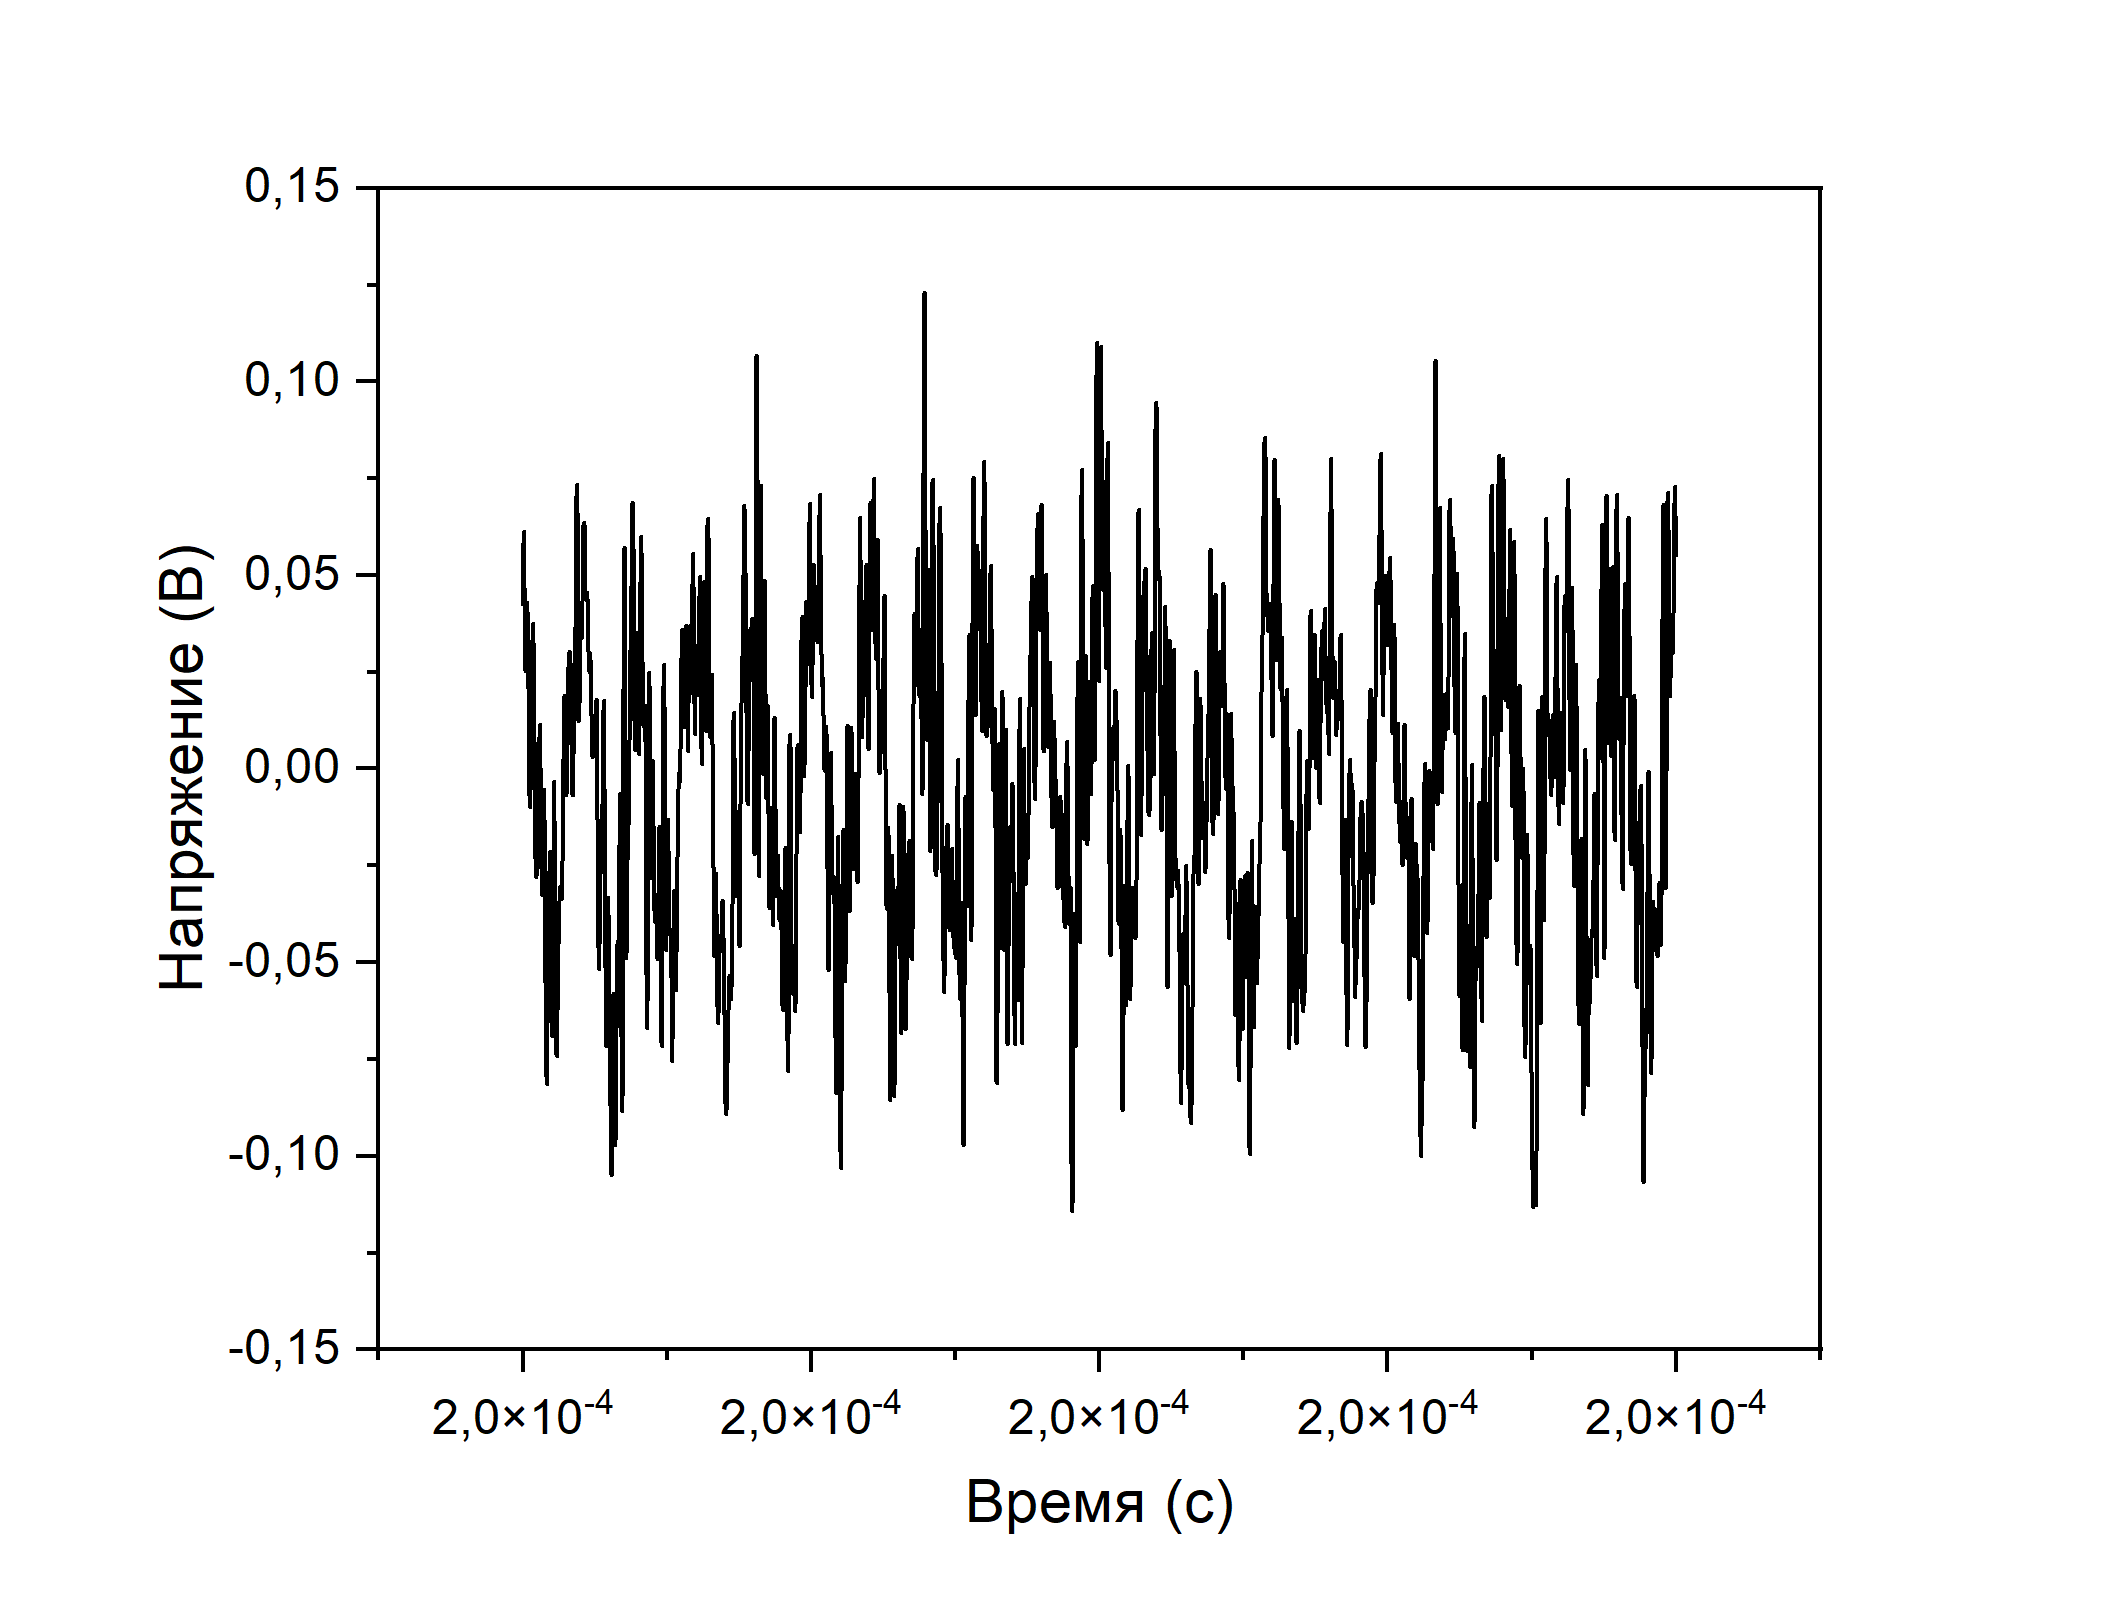
\includegraphics[width=\textwidth]{images/03.png}
    \caption{Noisy signal at the output of a balanced detector}
    \label{fig:noisy output inject syn}
\end{figure}
The received oscillation at the output of the balance detector carries phase information encoded by Alice. This signal is processed by digital signal processing techniques to extract the phase value of the signal. 
\begin{figure}
    \centering
    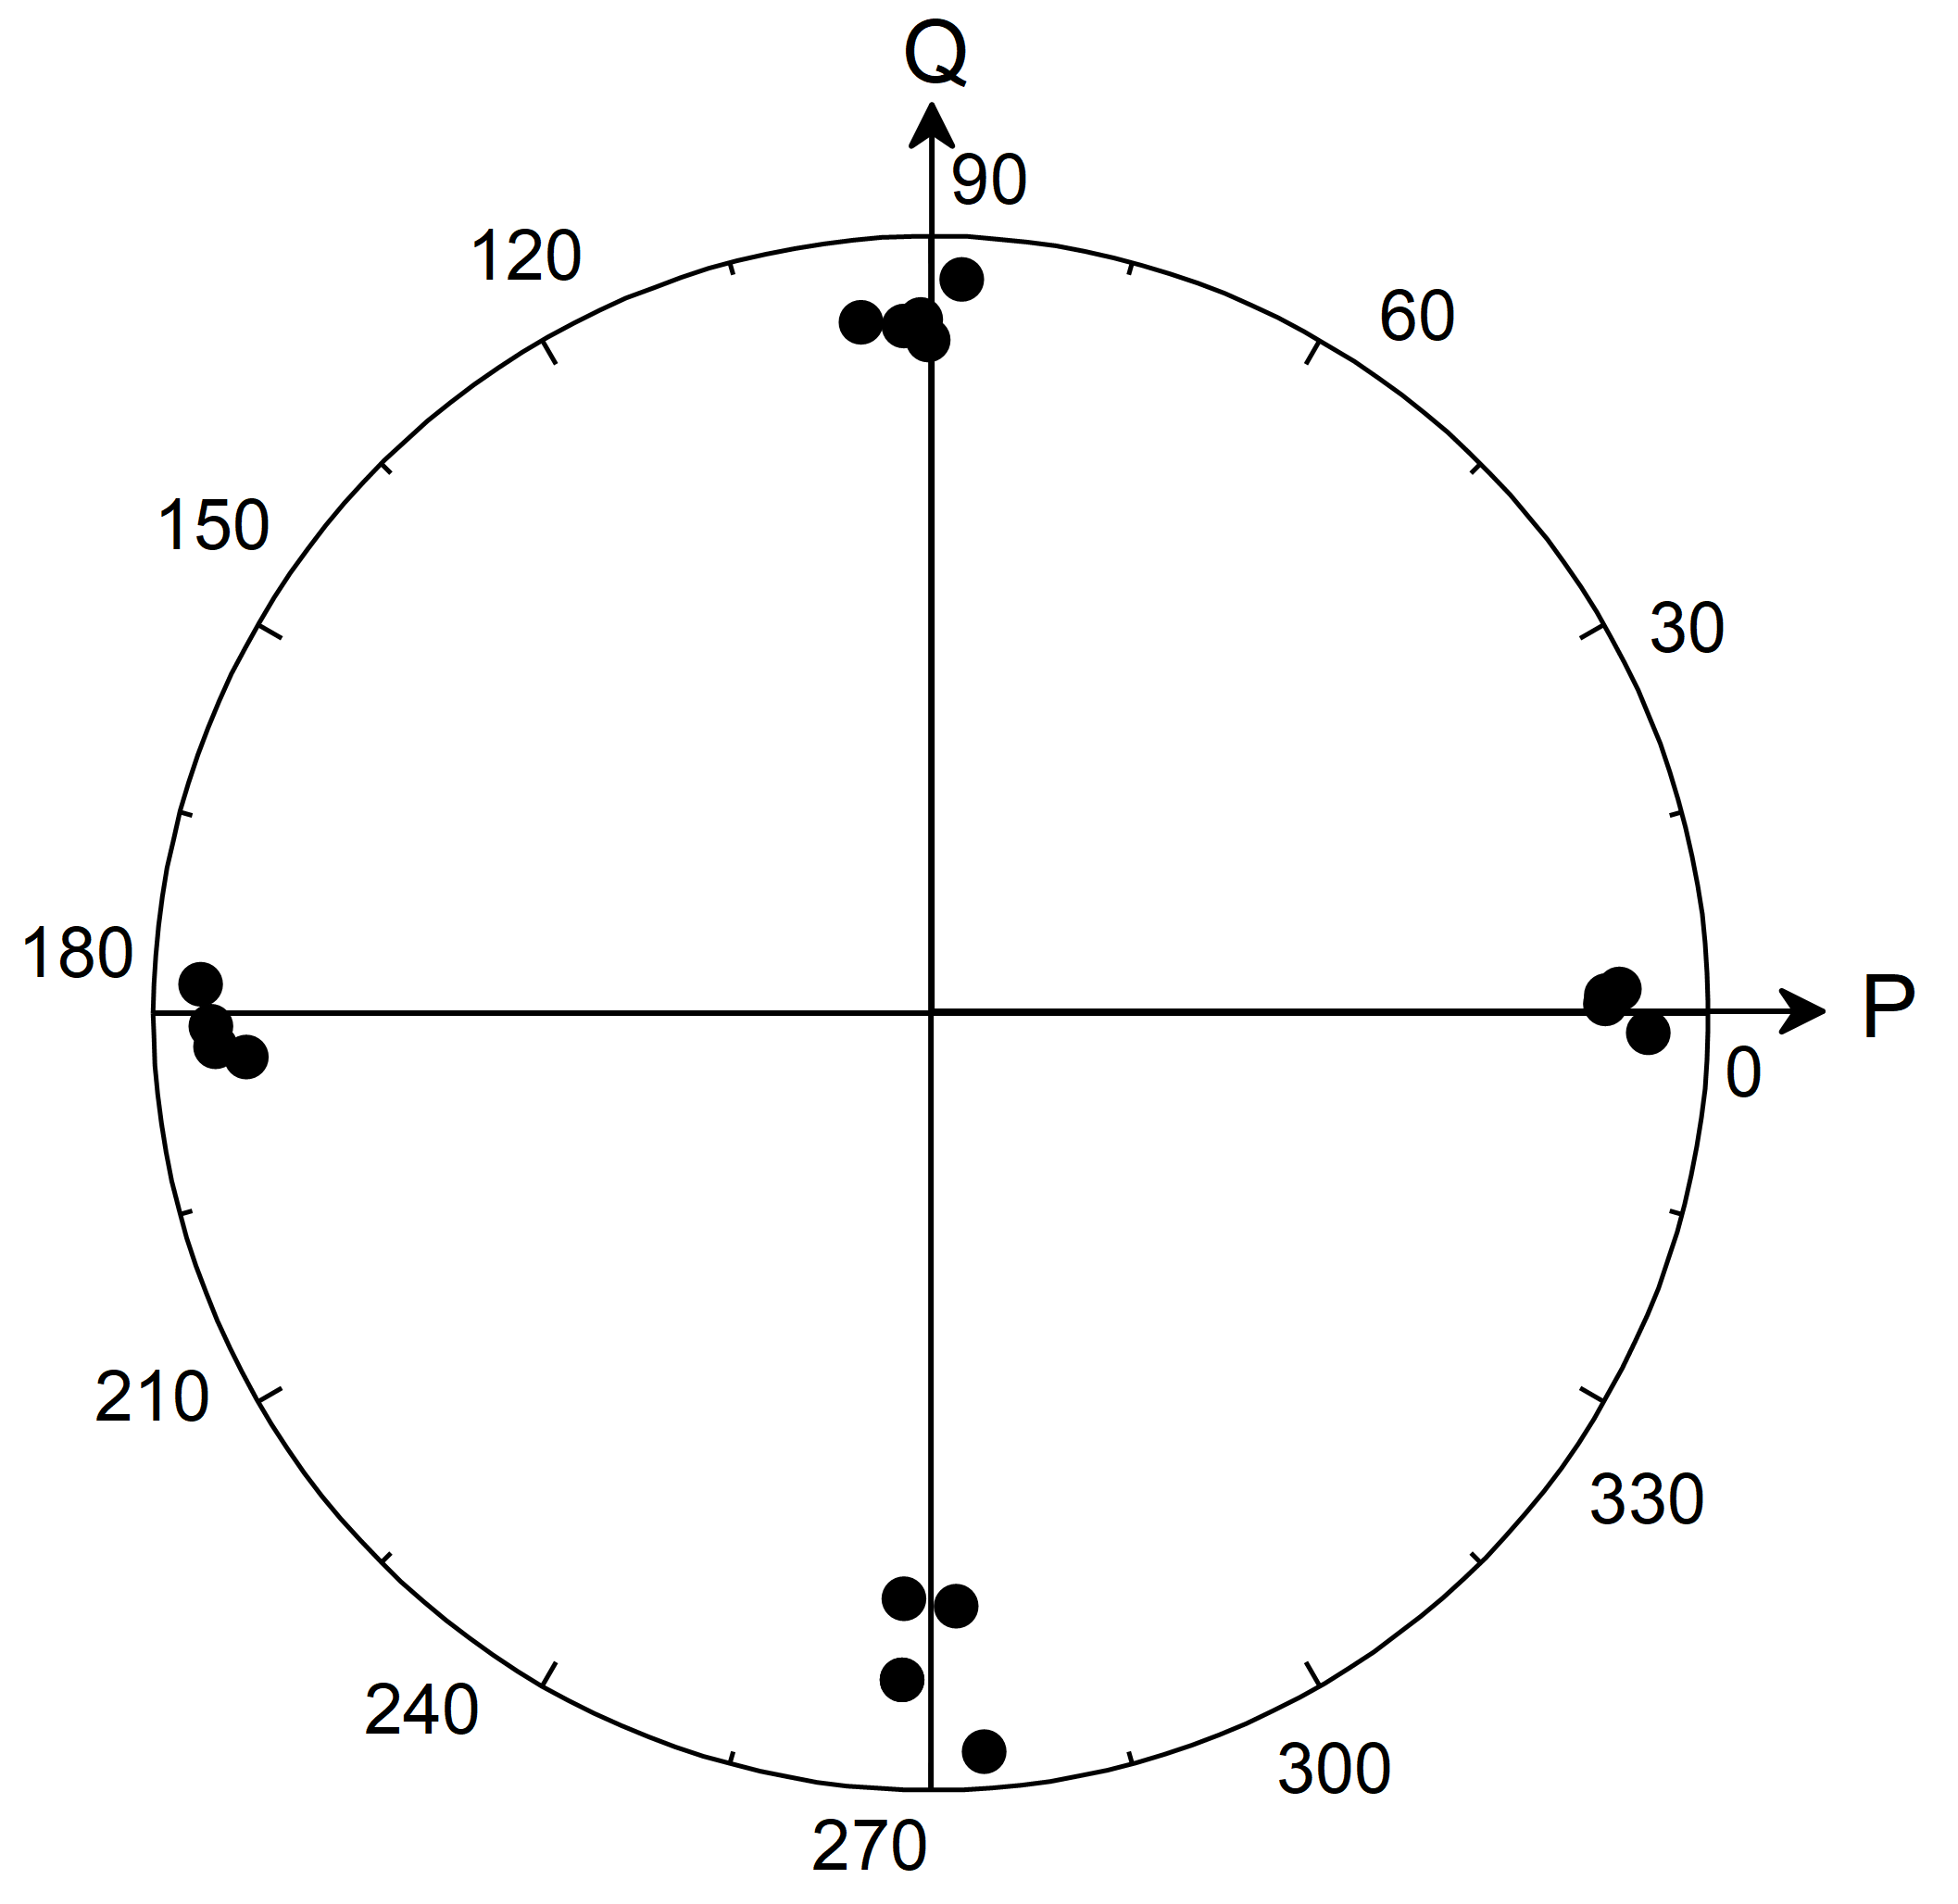
\includegraphics[width=0.8\textwidth]{images/06.png}
    \caption{Phase values obtained after digitalisation}
    \label{fig:phase meas ijnect syn}
\end{figure}

The resulting bit sequence is the raw key. The received key is sifted. In the obtained sifted key, the quantum bit error rate (QBER) is estimated by first opening a part of the key. And the last step is secrecy amplification using HASH functions.
To the pluses of this method of realisation of the QKD can be attributed the simplicity of the system, due to the fact that there is no active selection of the basis in the form of a modulator of any type. The presence of feedback in the form of optical injection allows to solve several problems: stabilisation of the LO wavelength, which also simplifies the final system, and reduces phase noise associated with the randomness of the phase of laser radiation generated by different sources. The use of heterodyne method of reception allows to use any type of modulation, which allows to flexibly adjust the protocol for different tasks and leaves the future for increasing the speed of key generation.
\newline The disadvantages of this system include the need for an additional fibre-optic communication channel for feedback, which is partially offset by the fact that real QKD systems are embedded into existing data transmission systems that work with multiplexing technology and the optical injection signal can be embedded into already used channels, as it has no requirements to the level of third-party noise. The second drawback, however, is the vulnerability to laser seeding attack, which requires further study and countermeasures. 
\newpage In the \underline{third chapter}, a scheme for applying the heterodyne detection method to detect \cite{brunner2017,delange1968,kuri2003} signals with two independent signal sources \cite{hajomer2024,shao2022} for a quantum communication protocol at side frequencies is discussed. A feature of this system is the transfer of quantum states of light to side frequencies that appear in the emission spectrum. The basic implementation of this protocol involves the use of discrete variables and single photon detectors based on avalanche photodiodes for signal registration. However, it is possible to adapt this protocol to use coherent detection methods\cite{samsonov2021,fadeev2024}. 
\newline In this paper we propose the use of heterodyne signal detection method for a quantum communication system at side frequencies.
\begin{figure}
    \centering
    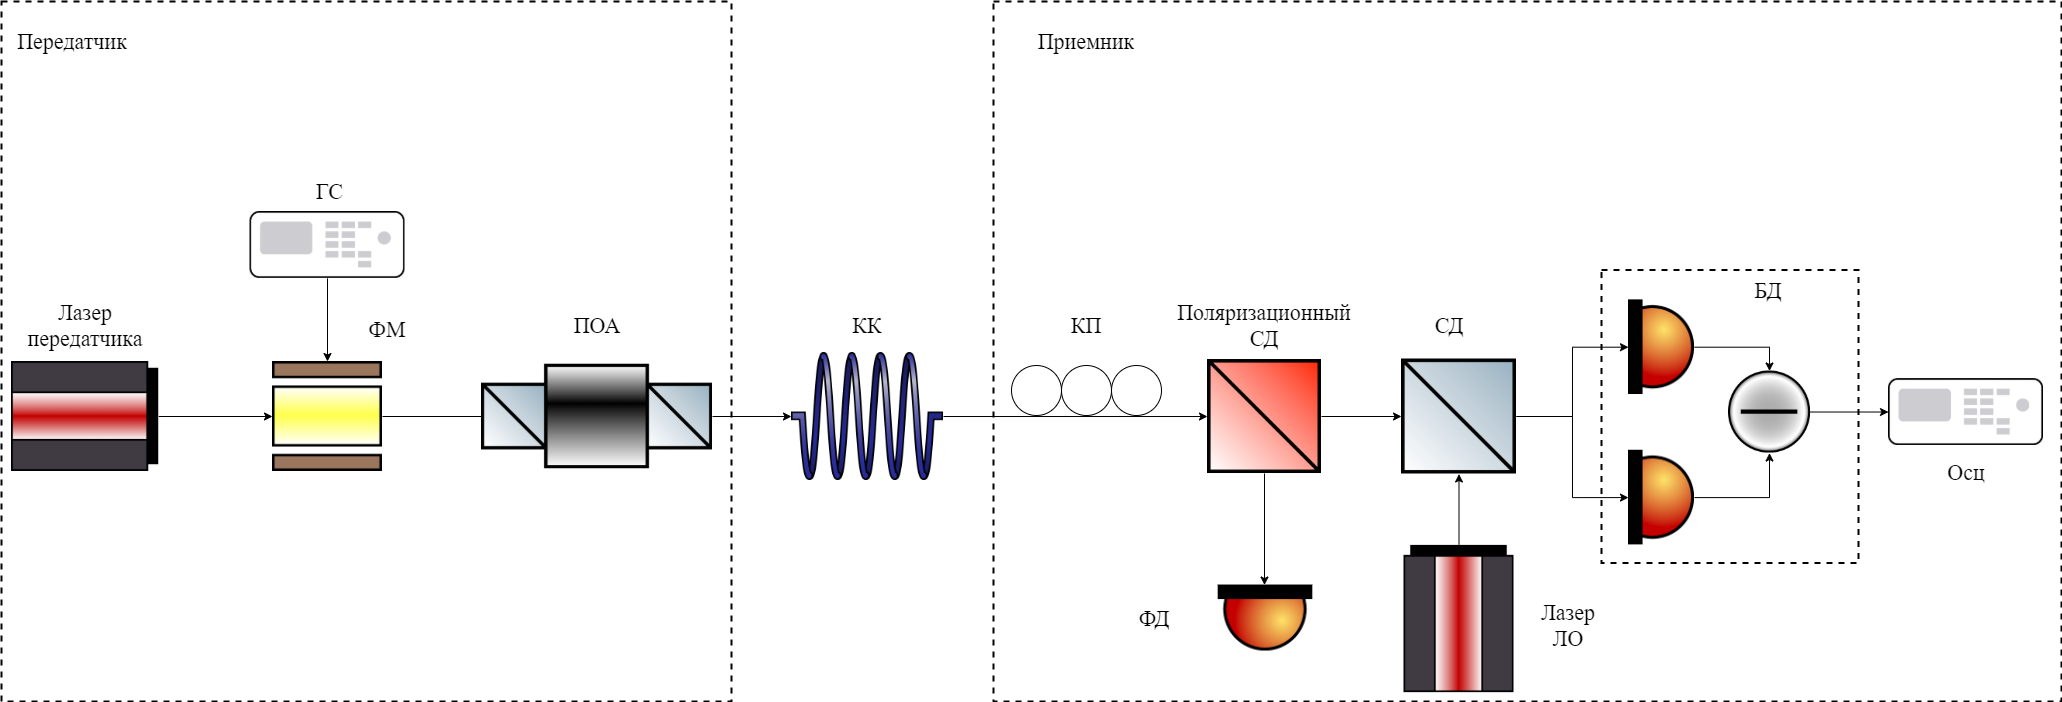
\includegraphics[width=\textwidth]{Гетеродин схема новая2 .png}
    \caption{Scheme of a quantum key distribution system at side frequencies with an independent local oscillator. SD - beam splitter, FM - phase modulator, GS - signal generator, POA - tunable optical attenuator, QC - quantum channel, BD - balance detector, Osz - oscilloscope}.
    \label{fig:het true scheme syn}
\end{figure}
This system works as follows. A laser on the transmitting side generates coherent radiation. This radiation, having passed through the necessary passive elements in the form of optical isolators, reaches the crystal of the phase modulator. An alternating voltage at the modulation frequency is transmitted to the electrical input of the phase modulator. A phase shift is introduced into this voltage, which corresponds to bits of information. Quadrature phase-shift keying or quadrature phase-shift keying (QPSK) is used as an example in this paper. The phase shift values in this case are {45\textdegree, 135\textdegree, 225\textdegree and 315\textdegree} and the following information bits {00, 01, 10, 11} correspond to these phase shifts. As a result of this modulation, three harmonics appear in the spectrum of radiation after the phase modulator, two of which encode information from the transmitter. The prepared radiation is attenuated by a variable attenuator to achieve a power level at side frequencies less than 1 photon on average. The quantum states thus obtained are transmitted via a fiber optic communication line to the receiving side.  
\newline The transmitted signal from Alice, after passing through the fiber optic link, reaches the polarization controller to compensate for the distortions introduced by the passage through the fiber. After that, the polarization beam splitter is installed and only the desired polarization is selected and the radiation with the desired polarization is allowed to pass through. The quantum states are then mixed with the LO generated by a separate laser on a beam splitter with two inputs and two outputs and a 50:50 splitting ratio. These signals interfere and as a result of this interference, the emission spectrum is enriched with additional harmonics. These harmonics appear because the frequencies of the LO and the Alice laser do not match. These spectral components are at different frequencies - total, difference and Raman. But given the limited bandwidth of the balance detector, we can observe at its output only harmonics at difference frequencies that fall into it. Total and other combinational frequencies do not fall into the bandwidth of the DB and are registered as a constant component, which loses all the information encoded in their phases. Where as the harmonic oscillations at the difference intermediate frequency pass the amplifying stage unchanged and retain the information encoded in the phase of Alice's emission. In this way, the spectrum is transferred from the optical domain to the radio frequency domain, where amplification and signal processing are simplified.
\begin{figure}
    \centering
    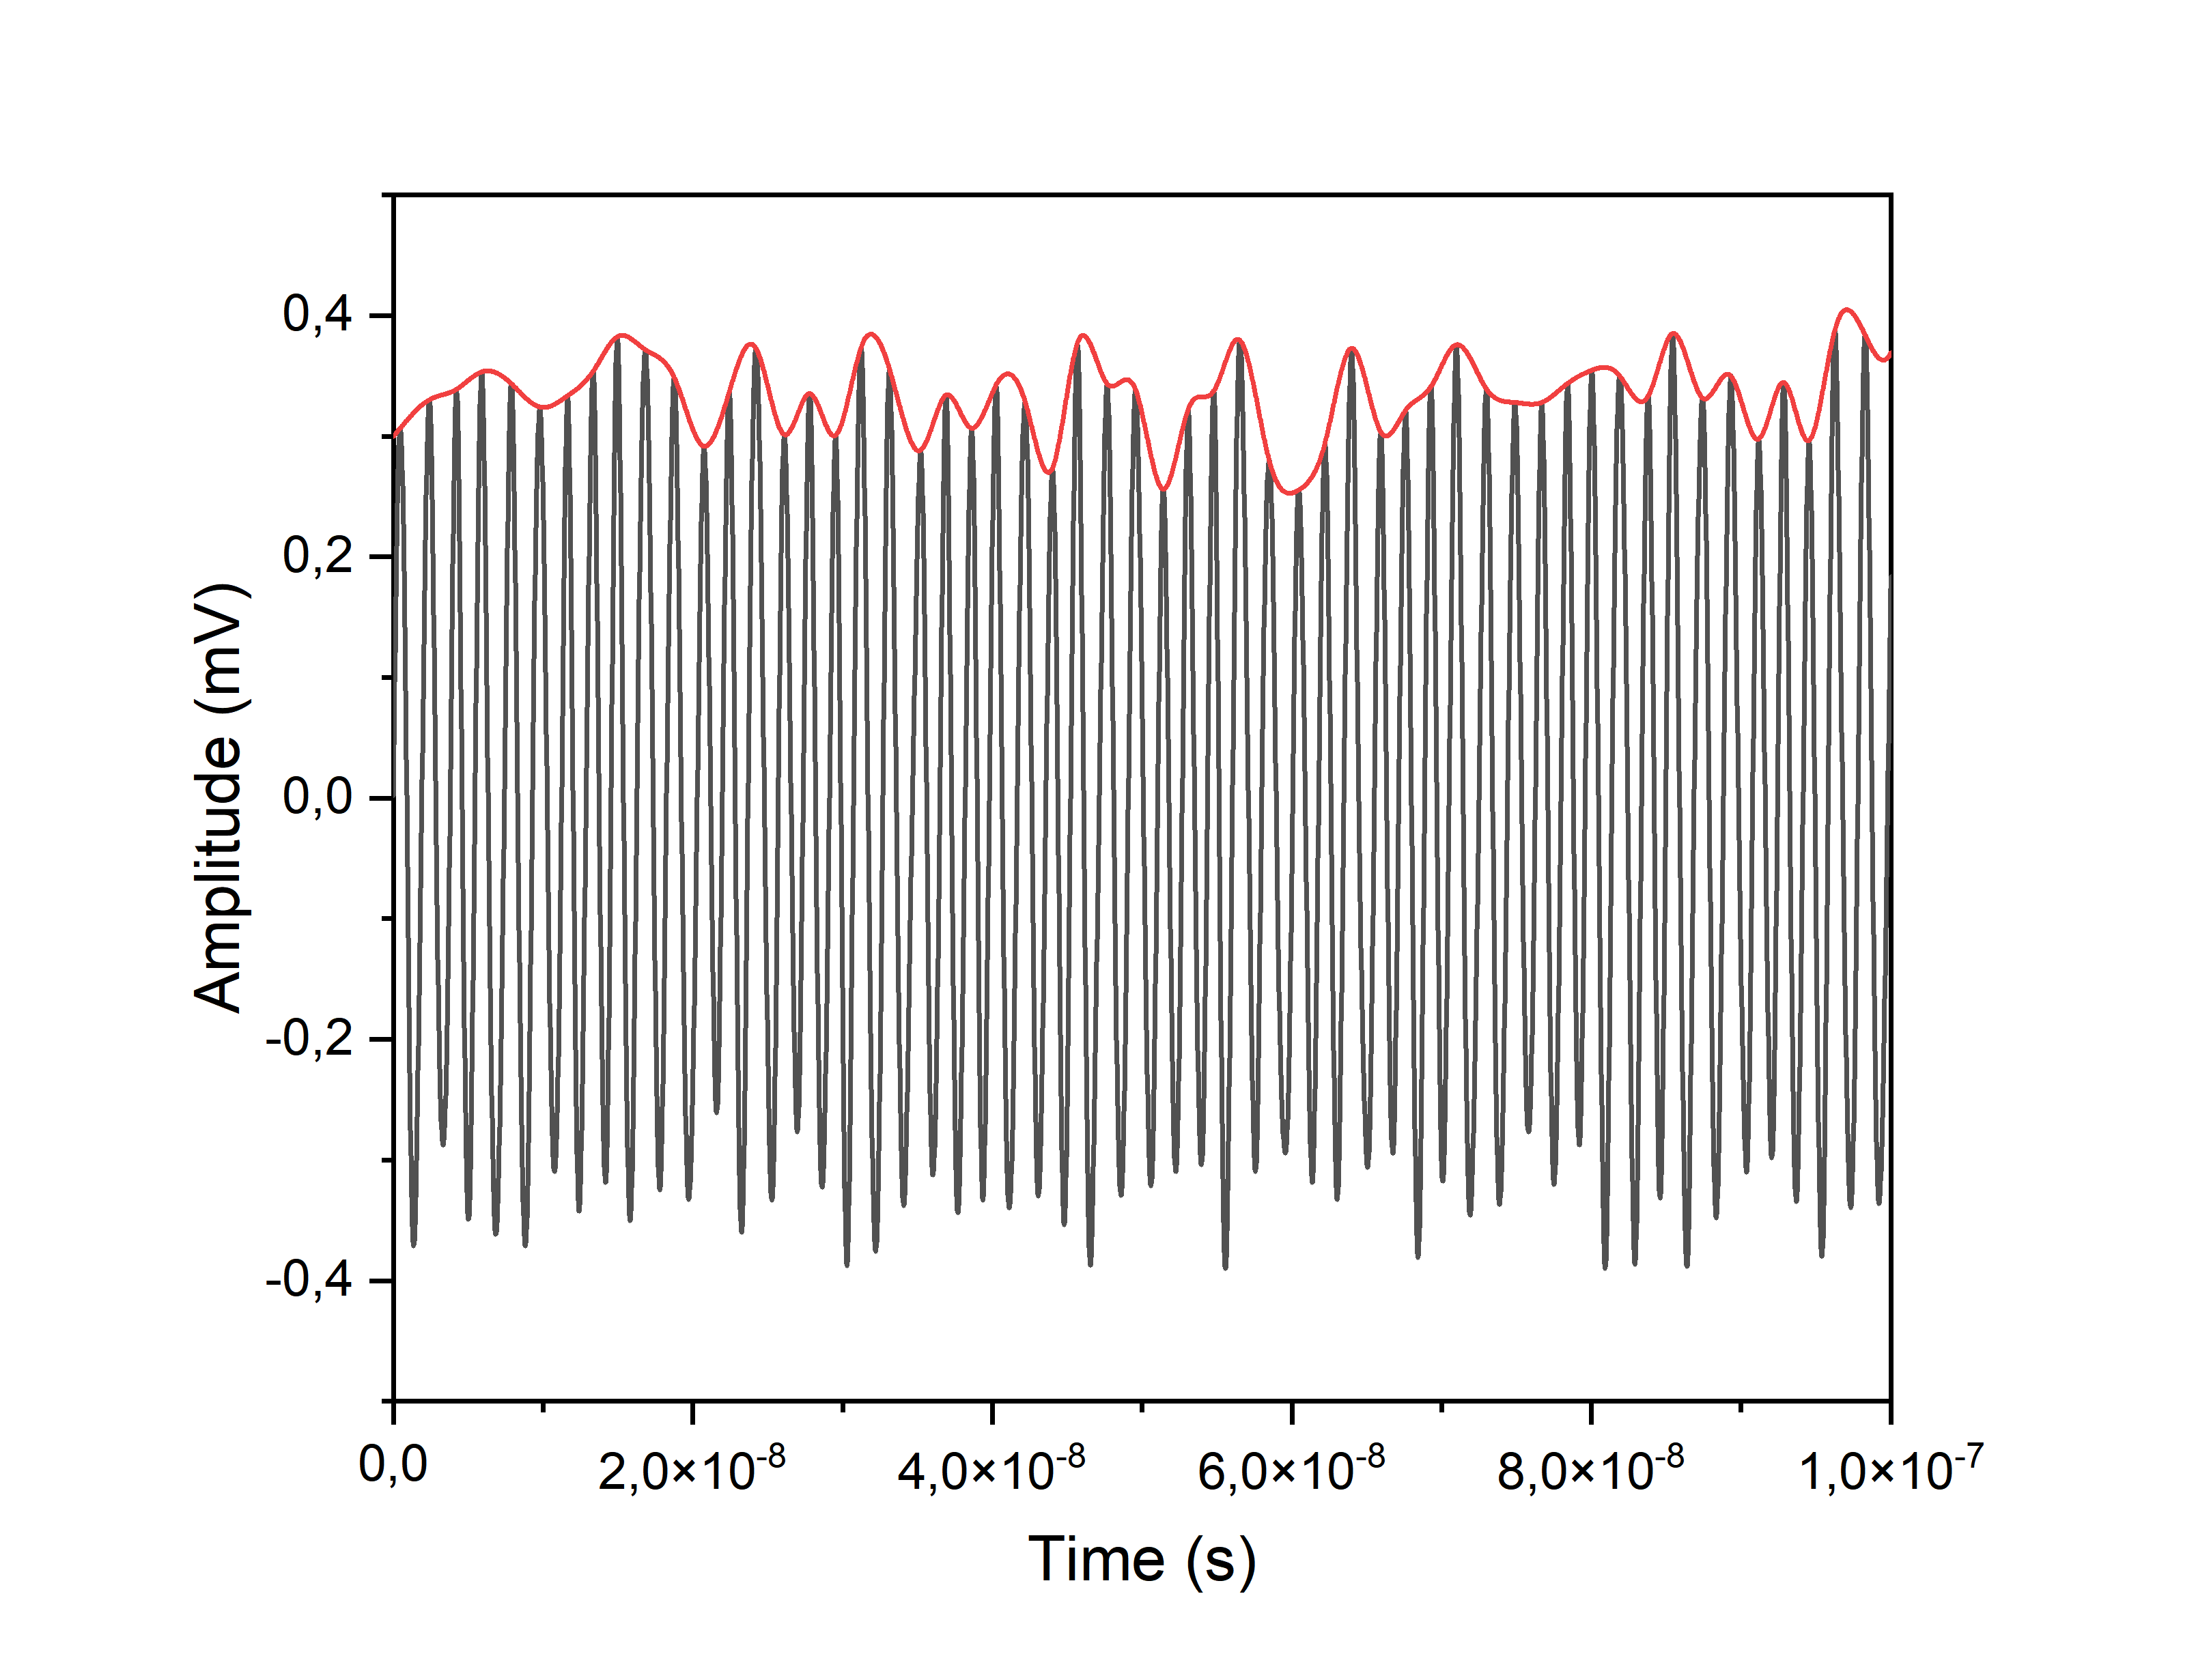
\includegraphics[width=\textwidth]{images/balanced output heterodyne.png}
    \caption{The signal at the output of the balanced detector after heterodyne reception}.
    \label{fig:het time output syn}
\end{figure}
\newline A balance detector is a device that consists of two photodetectors connected so that their photocurrents are mutually subtracted. The received signal is then filtered to eliminate the influence of the constant component of the photocurrent. After that the received signal goes to the amplifier stage to increase its amplitude. The presence of the amplifier stage limits the bandwidth of the entire device. Typical bandwidths can vary from 100 MHz to 1.2 GHz. This limits the range of received frequencies and the raw key generation rate. 
\newline The received signal after amplification must be digitised by an ADC for further processing. As processing can be applied various methods of digital signal processing, such as Fast Fourier Transform or Hilbert Transform. As a result of this processing, phase values are generated from the harmonic signal received after the ADC, which correspond to given bit values from which a bit sequence called raw key is formed. 
However, using LO at the receiver side requires tweaking its polarisation and the polarisation of the quantum states for effective interference at the receiver. In this work, a polarisation control algorithm based on Fast Fourier Transform is proposed. The essence of this algorithm is that when a polarisation beam splitter is used, the modulation frequency that carries the information from the transmitter is doubled.
This appearance of the doubled frequency can be tracked in the frequency domain. The following algorithm is used for this purpose 
\begin{enumerate}
    \item Apply FFT to the received signal
    \item Analyse the spectral composition of the signal
    \item Rotating the polarisation of the signal until the harmonic is eliminated at twice the modulation frequency.
    \item Further rotation of the signal polarisation to the harmonic maximum at the modulation frequency
\end{enumerate}
As a result of its operation, it is possible to adjust the polarisation by using active polarisation control, which will use the FFT result as feedback to adjust the polarisation. 
\begin{figure}
    \centering
    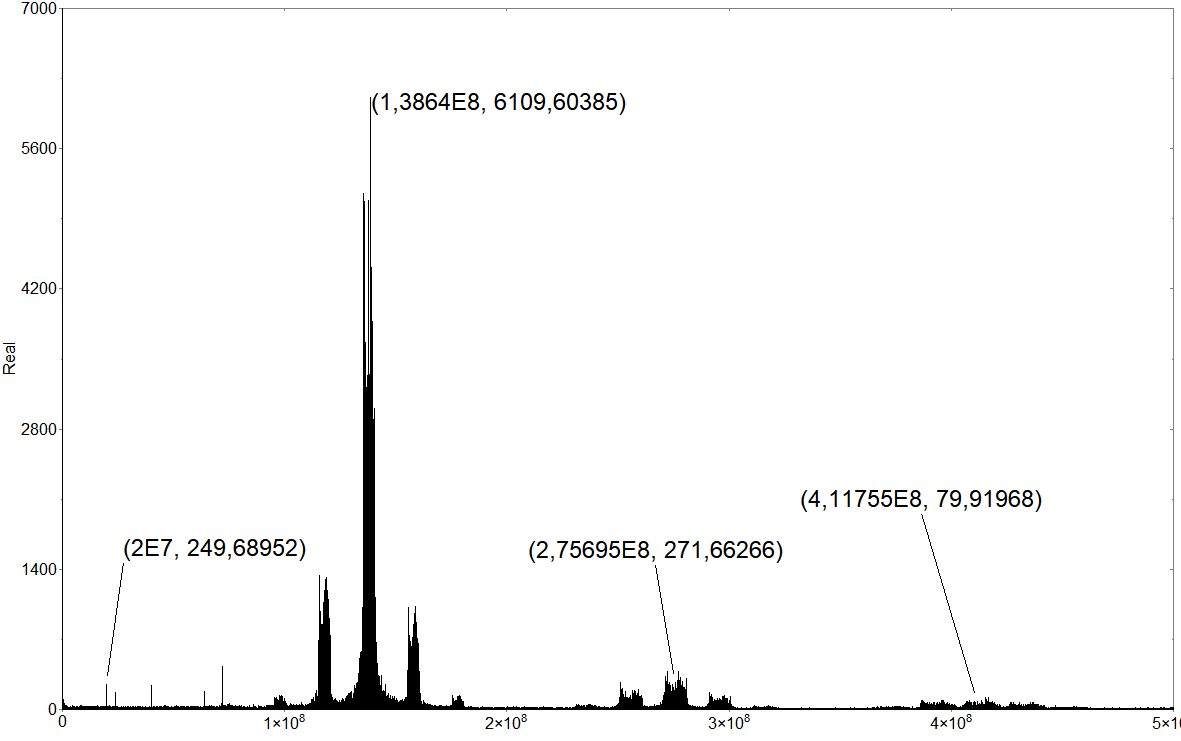
\includegraphics[width=\linewidth]{Spectrum of ruined polarization.png}
    \caption{Spectrum of ruined polarisation}
    \label{fig:ruined pol syn}
\end{figure}
\begin{figure}
    \centering
    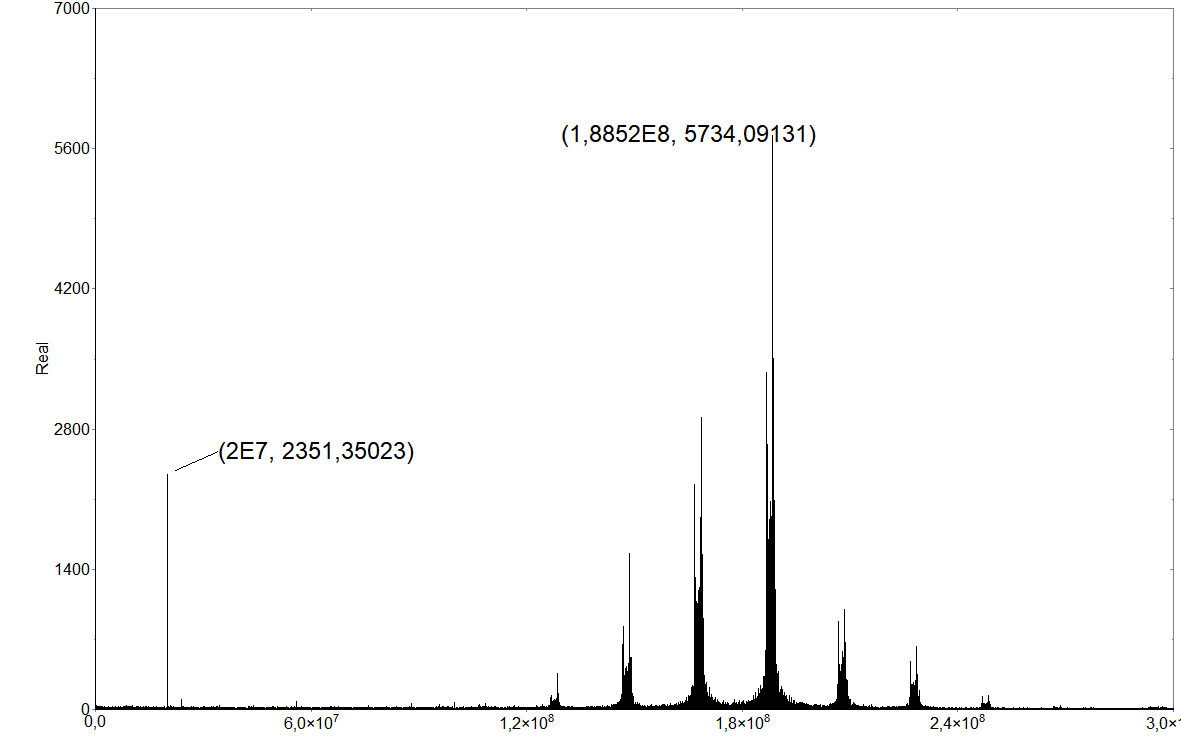
\includegraphics[width=\linewidth]{normal polarization.png}
    \caption{Spectrum of a signal with distorted polarisation}
    \label{fig:norm pol syn}
\end{figure}
Figure~\ref{fig:ruin pol syn} shows the spectrum of an information signal with distorted polarisation. The information about the presence of a doubled modulation frequency is fed to the polarisation controller and it starts its operation until the true modulation frequency is maximal and the doubled modulation frequency disappears. The result of the algorithm is shown in Figure~\ref{fig:syn norm pol}. The spectrum of the signal at normal polarisation contains no harmonic at the doubled frequency and the harmonic at the modulation frequency is maximal.
\newline To the advantages of this method can be attributed flexibility in the choice of protocol, as the transfer of information to the intermediate frequency allows you to analyse almost any modulation without the need to introduce additional elements, for example, phase modulator to select the basis. The use of two independent sources of coherent radiation allows not to use feedback systems, which require an additional optical channel and open additional opportunities for an intruder. Generation of a local oscillator on the receiver side allows to increase its power, compared to protocols in which LO is transmitted over a quantum channel, which allows to reduce noise associated with scattering in the FOCL and increase the signal-to-noise ratio, which positively affects the bit rate.
\newline From the disadvantages of the same can be highlighted the need to adjust the frequency, as two independent oscillators need periodic frequency adjustment. This problem is solved by the peculiarity of the protocol of quantum communication at side frequencies due to the fact that in the spectrum there is a powerful carrier, which is also knocked down with the local oscillator and is transferred to an intermediate frequency. By analyzing this frequency after FFT processing, it is possible to adjust the LO frequency so that all signals fall within the bandwidth of the balanced detector. Another disadvantage is the random phase noise due to the randomness of the laser generation process in two independent sources. This problem is solved by analyzing the phase of the intermediate frequency between the local oscillator and the optical carrier obtained after Alice phase modulation. This signal will contain the phase noise of both the LO and the transmitter laser, which can be accounted for in post-processing by pre-processing with digital methods. 
\newpage \underline{Chapter Four} is devoted to the study of the effect of the intruder radiation at a wavelength of 1310 nm on the source of coherent radiation based on a semiconductor laser diode with distributed feedback. This vulnerability in its technical implementation is called optical pumping attack\cite{fadeev2024b,fadeev2025}. This type of attack is similar to the Laser Seeding attack\cite{huang2019,lovic2023} in that Eve injects its radiation into the laser resonator on the transmitter to alter its characteristics. However, there is a significant difference. In the case of a seeding attack, the attacker uses the same or close wavelength to the operating wavelength of the laser under attack. Whereas in the case of an optical pumping attack, Eve uses a laser wavelength that differs by 50 nanometers or more from the operating wavelength of Alice's laser. This feature makes it possible to more effectively circumvent countermeasures using passive fibre-optic elements in the form of isolators\cite{borisova2020,nasedkin2022,nasedkin2023}. Their isolation coefficient has a spectral dependence, which leads to the fact that the insertion isolation at 1310 nm wavelength is significantly smaller than at 1550 nm wavelength. As a result, the attacker requires less probing power to achieve the desired effect. 
\newline This attack is constructed as follows. The attacker installs a fibre circulator with three ports into the break in the fibre optic link. Eve's probing laser is plugged into the first port. The second port is plugged into the fibre optic link towards the sender side and the third port is plugged into the receiver side. In this way the intruder's radiation will enter the optical circuitry of the transmitter, and Alice's radiation will pass through the fibre towards the receiver without any problems. The intruder's radiation undergoes attenuation as it passes through the optical circuitry of the transmitter, so it is necessary to have sufficient probing power to make changes to the laser characteristics. The passed radiation enters the laser crystal and is absorbed in it\cite{hui2023}.
\begin{figure}
    \centering
    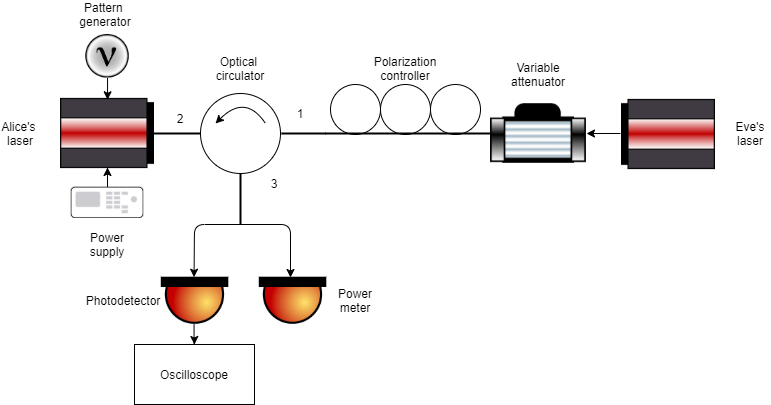
\includegraphics[width=0.75\textwidth]{images/1310 experiment.png}
    \caption{Schematic of the laser seeding experiment. Alice's Laser - Alice's Laser, Pattern generator - pulse sequence generator, Power Supply - laboratory power supply, optical circulator - optical circulator, polarisation controller - polarization controller, varriable attenuator - tunable attenuator, Eve's laser - intruder laser, Photodetector - photodetector, power meter - power meter, Oscilloscope - oscilloscope}.
\label{fig:exper 1310 syn}
\end{figure}
This causes an additional population inversion to be created, resulting in a shift in the Watt-Ampere characteristic of the laser while the pump current is unchanged.
\begin{figure}
    \centering
    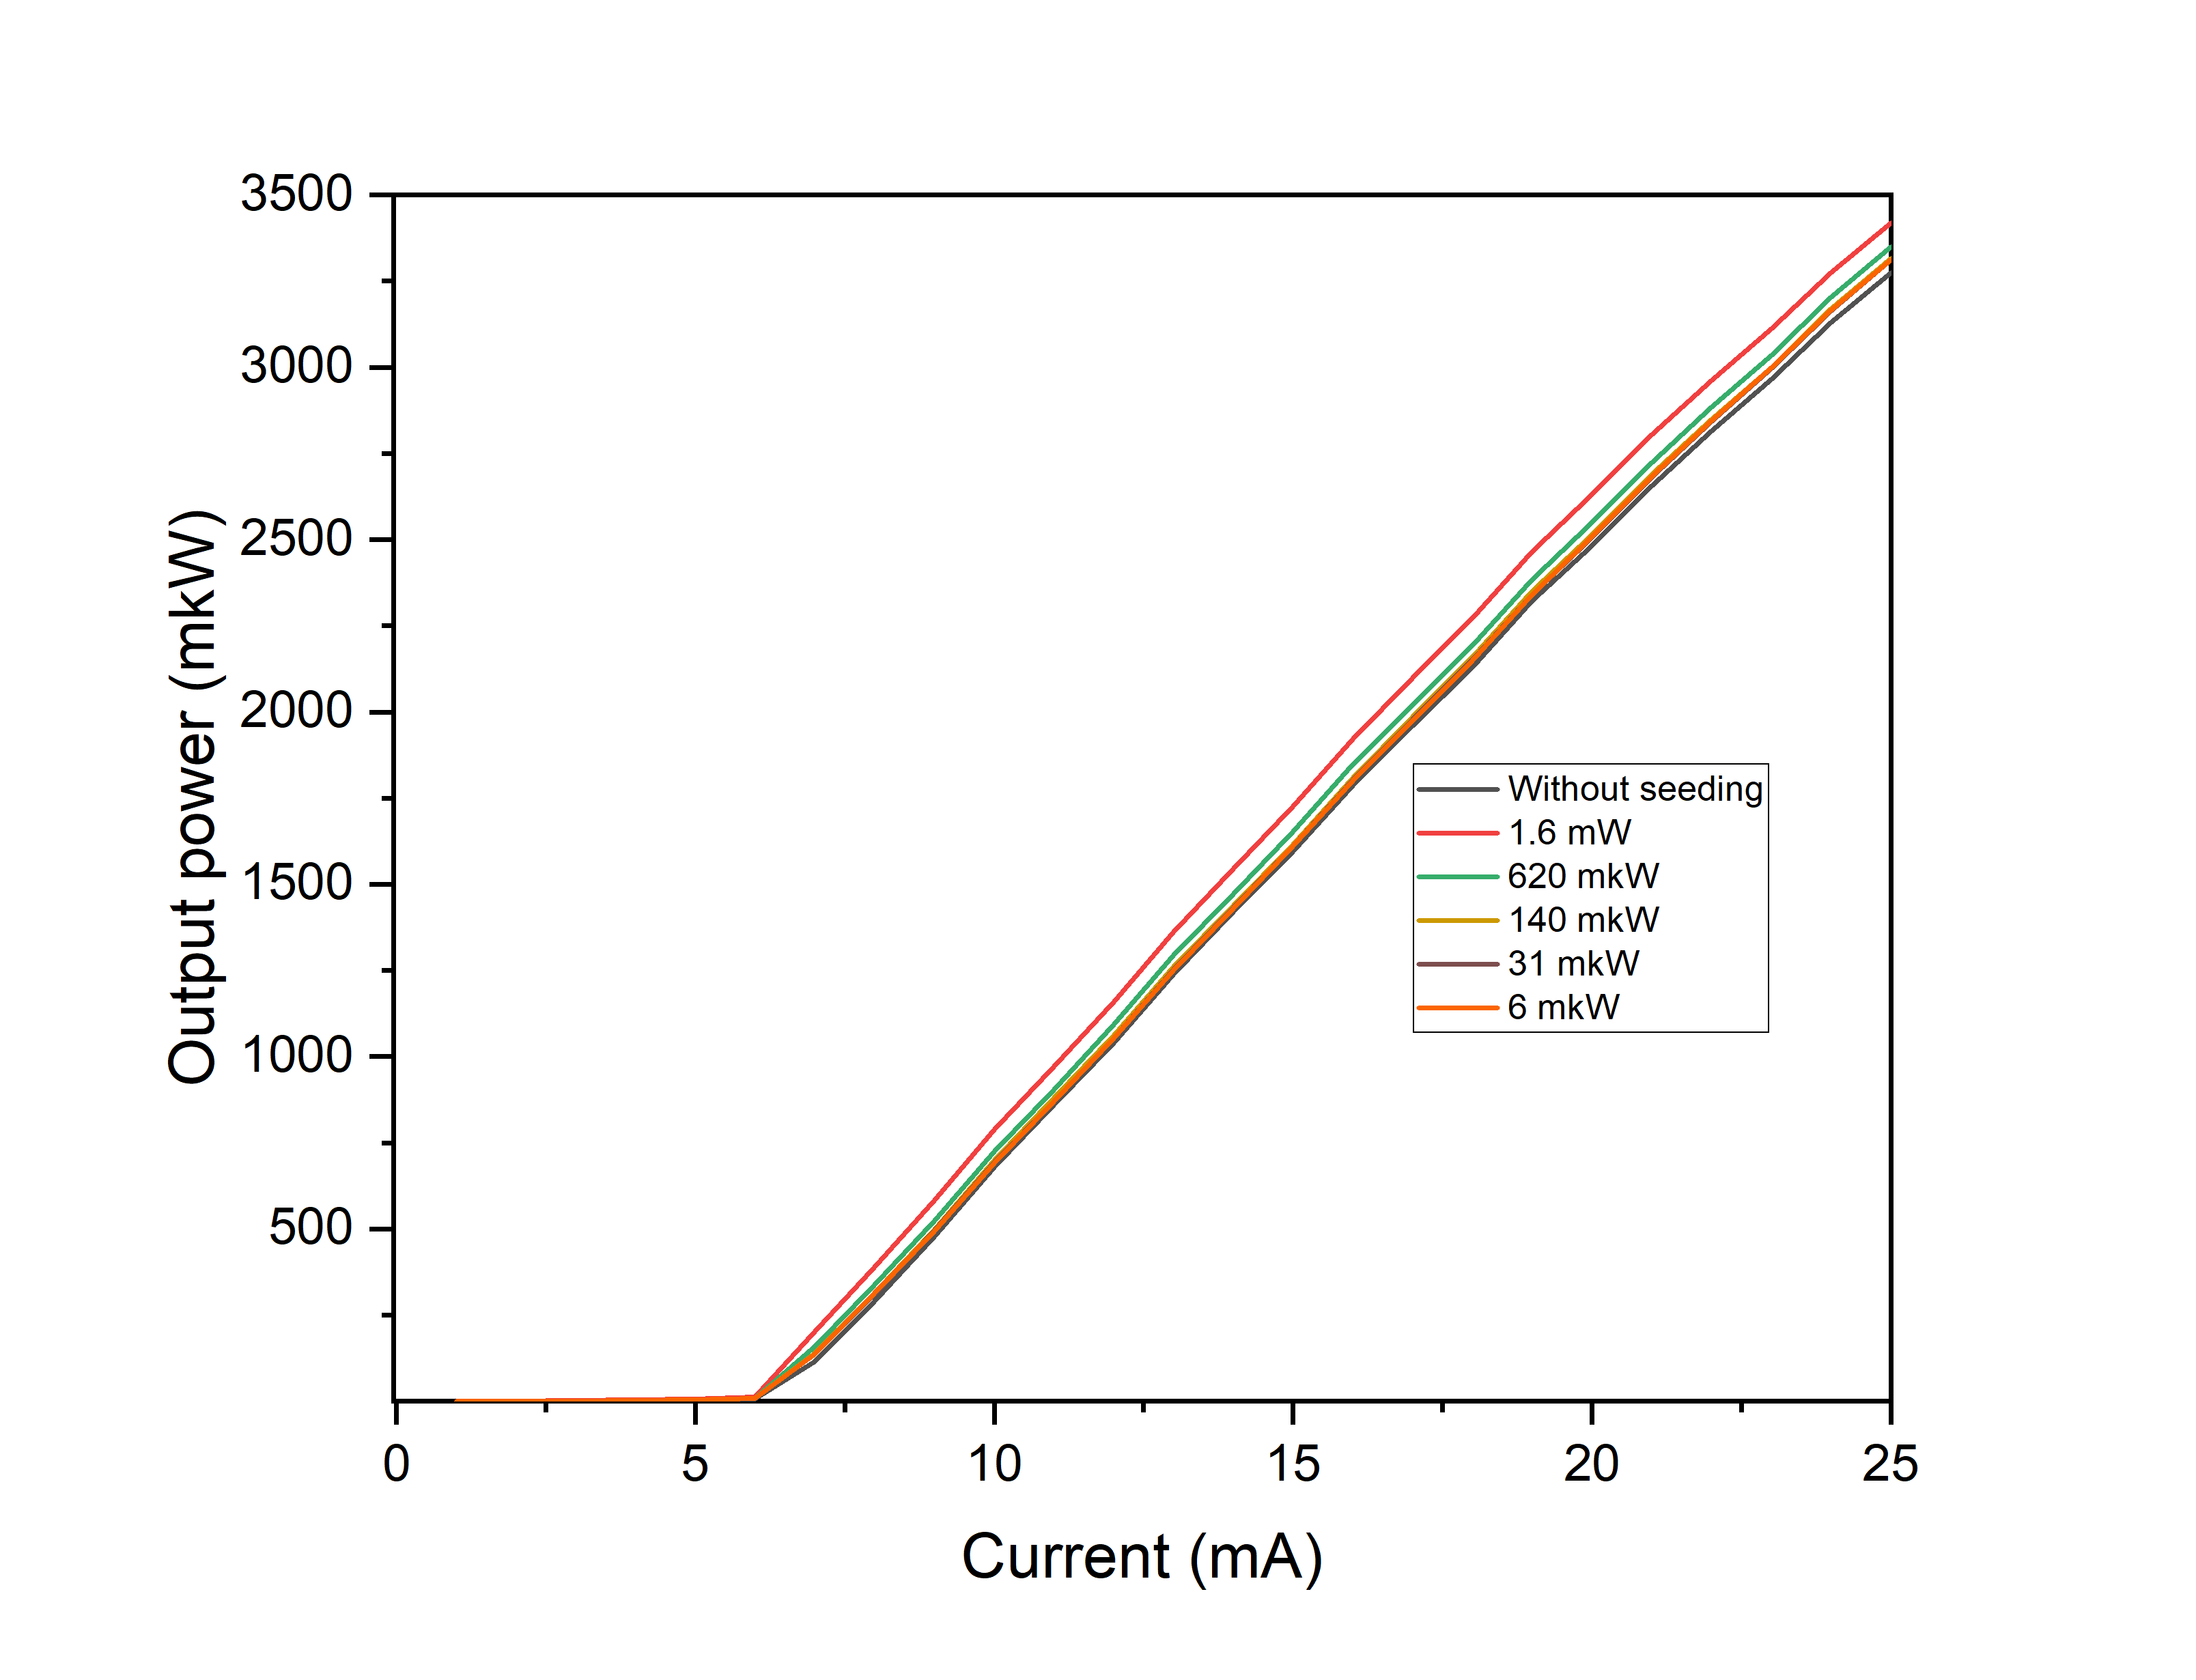
\includegraphics[width=0.75\textwidth]{images/ватт ампер для диссера.png}
    \caption{Variation of Watt Ampere characteristics under different pump powers at 1310 nm wavelength. Output power is output power in microwatts, current is current in milliamperes}
    \label{fig:watt-amp syn}
\end{figure}
This causes the calibrated radiation source on the transmitter side to start emitting more power than originally intended. As a result, this causes the output average photon number to increase, generating a larger number of multiphoton states, which opens up the possibility of realising a photon number splitting attack. The same effect is manifested in the change of the pulse shape. Optical pumping~\cite{svelto2010,okamoto2003,guina2017} increases the pulse area and, consequently, its energy, increasing both the average number of photons in signal pulses and the average number of photons in decoy states in the BB84 protocol with decoy states \cite{liu2020}.

\begin{figure}
    \centering
    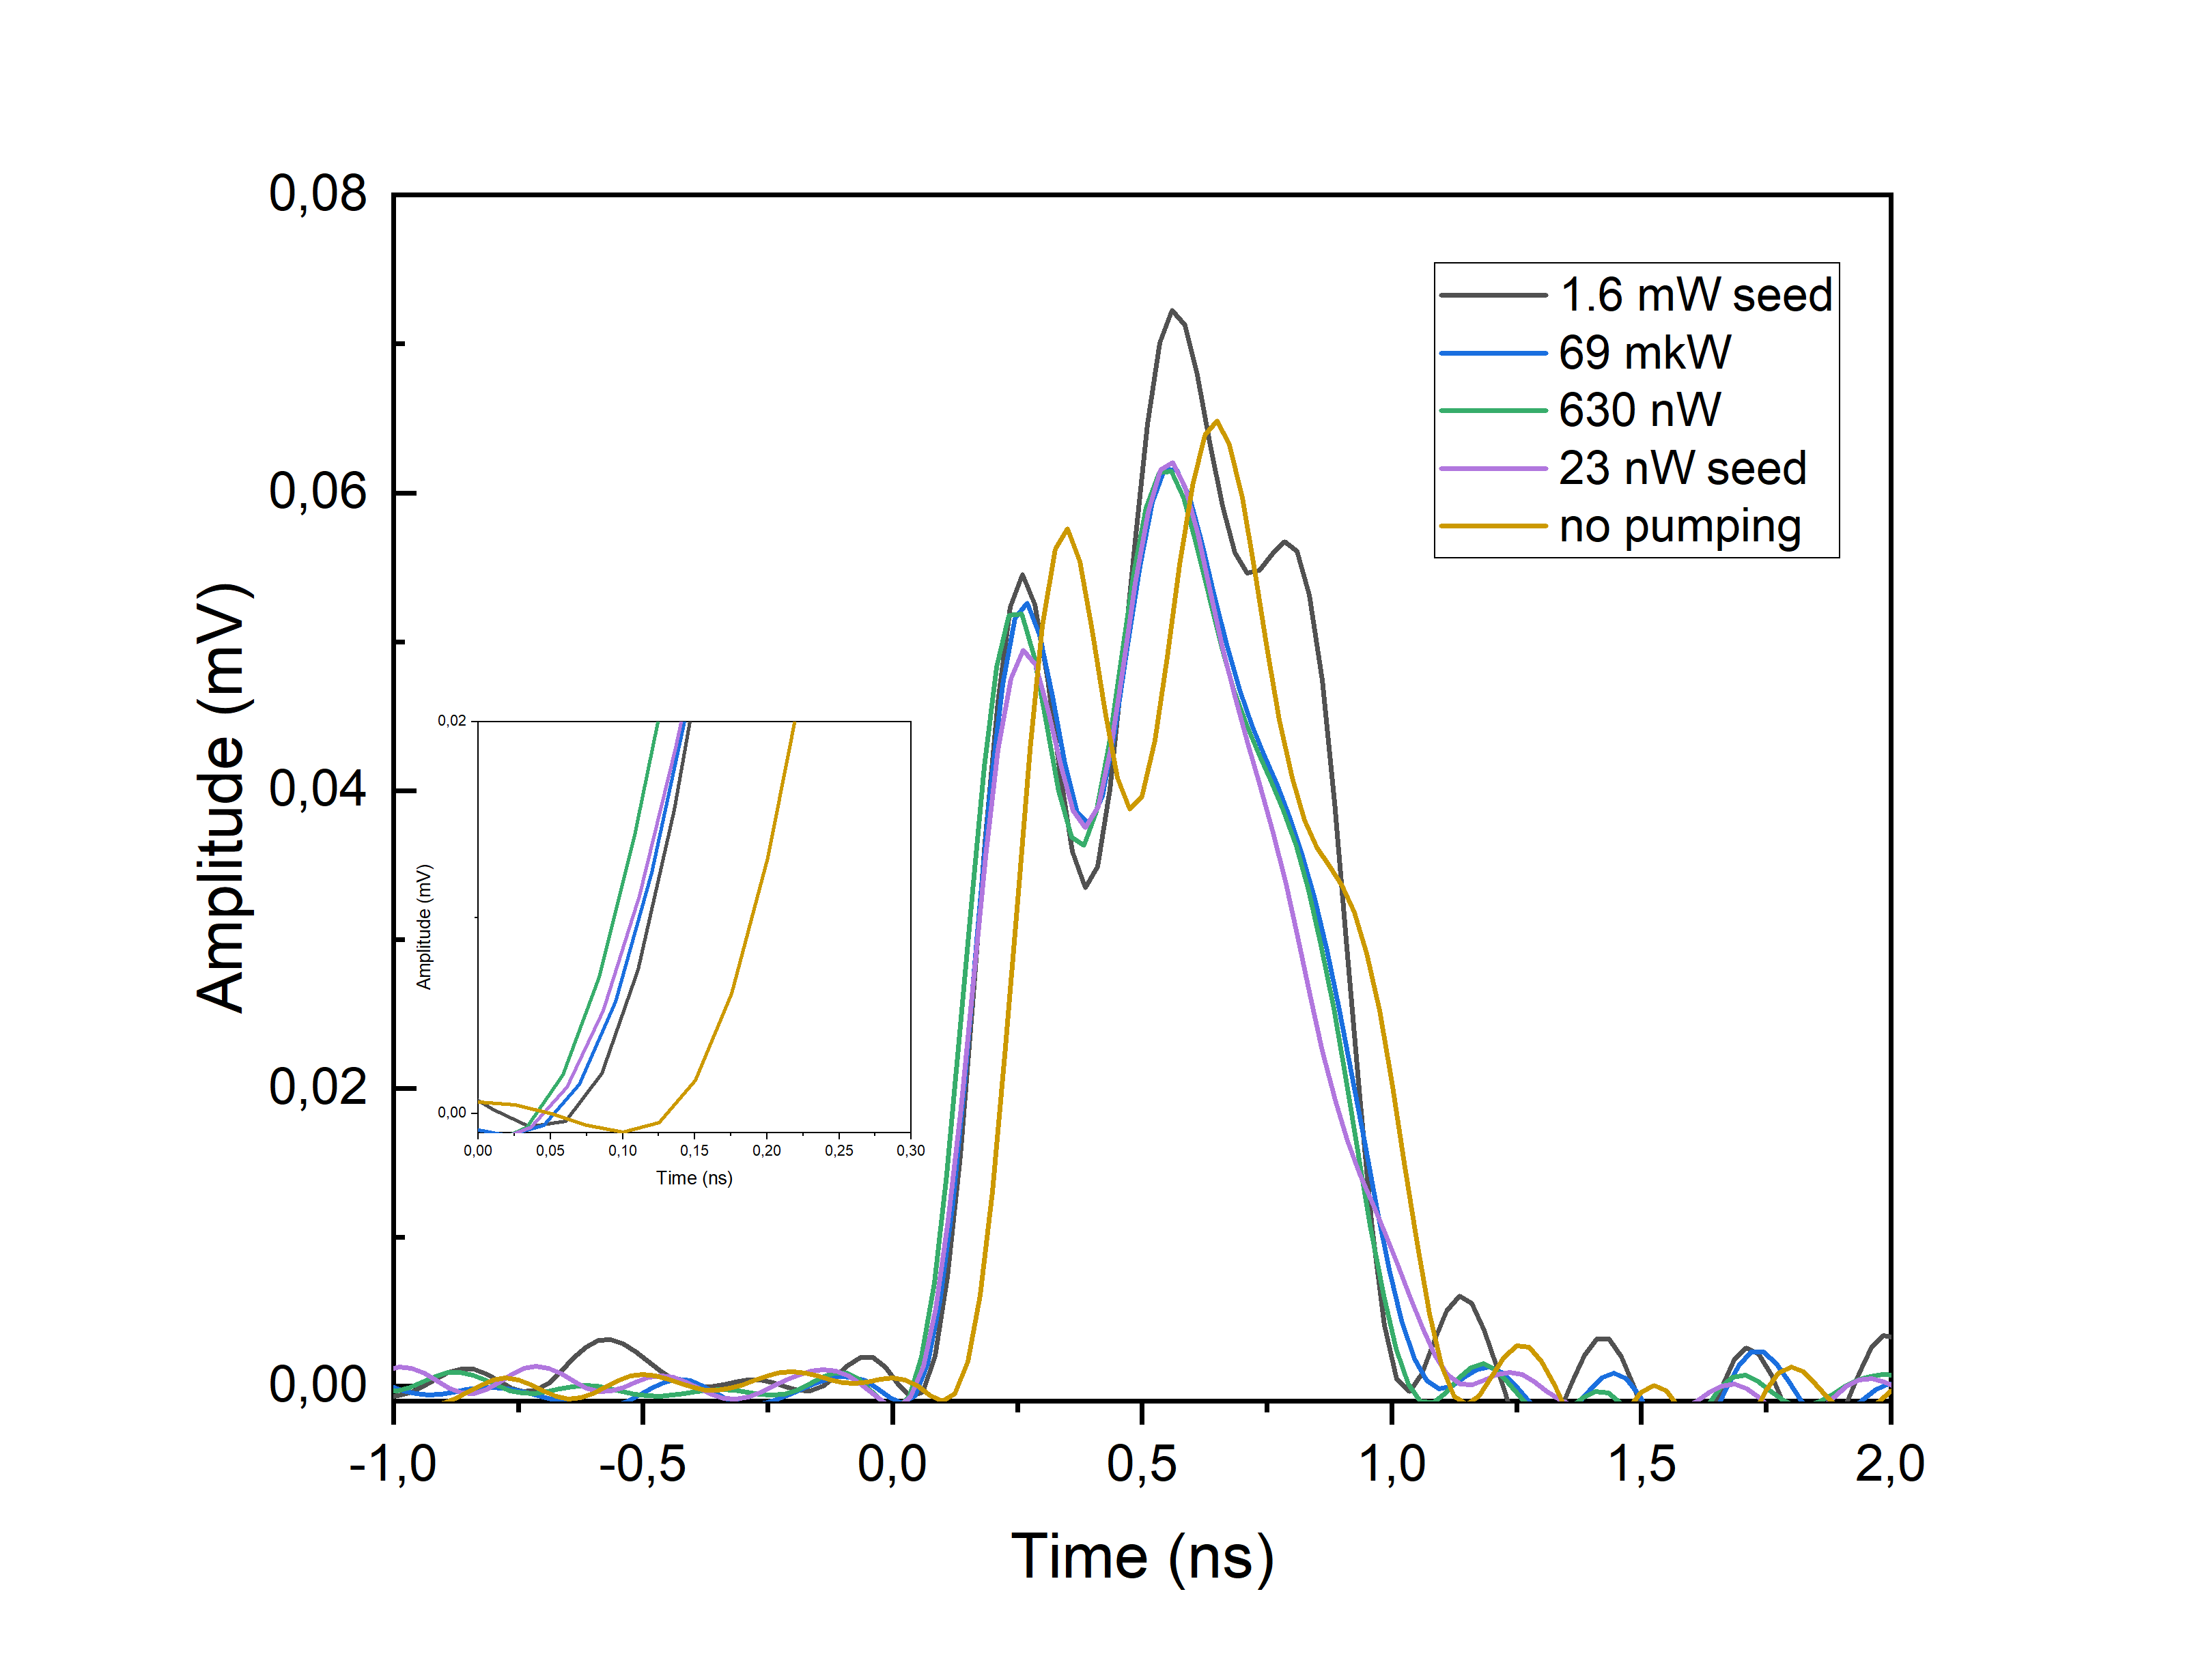
\includegraphics[width=0.75\textwidth]{images/Импульсы под действием 1310 для диссера.png}
    \caption{Change of pulse shape under the action of external optical pumping at different powers at the wavelength of 1310 nm. Amplitude is amplitude in millivolts, Time is time in nanoseconds, seed is seeding, and pumping is pumping}.
    \label{fig:pulses 1310 syn}
\end{figure}
\newpage In the framework of this work, we show the implementation of an optical pumping attack at a wavelength of 1310 nm, which leads to an increase in the laser output power at constant pump currents, an increase in the pulse area, and an increase in the quantum efficiency of the laser. These effects create conditions for other types of attacks on the QRC system. In the case of this work it was shown that a probing power of 200 $\mu W$ is sufficient to increase the quantum efficiency by 1\%, demonstrated in the graph \ref{fig:eff syn} and to increase the output power by $4\%$. The minimum power required for an attacker to effectively attack a typical optical transmitter circuit implementing the BB84 protocol was calculated.
\begin{figure}
    \centering
    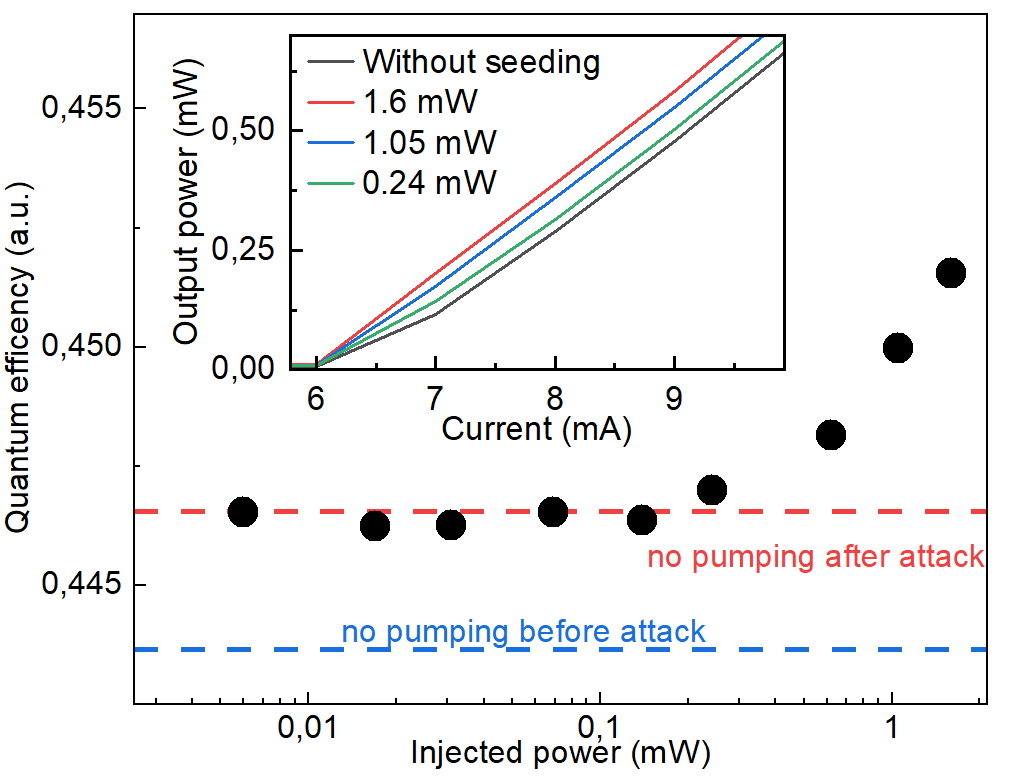
\includegraphics[width=0.7\textwidth]{images/Эффективность 1310.png}
    \caption{Change in quantum efficiency due to external radiation at 1310 nm wavelength. Quantum efficiency - quantum efficiency in relative units, Output power - output power in milliwatts, Injected power - injected power in milliwatts, current - current in milliamperes, blue dashed line - value of quantum efficiency before attack, red dashed line - value of quantum efficiency after attack. }
    \label{fig:eff syn}
\end{figure}
\newpage The research conducted in the \underline{chapter six} is devoted to the study of the effect of high-power coherent radiation on a laser source based on optical injection. Such sources are actively used in quantum communication systems implementing a protocol with an untrusted receiver node \cite{comandar2016,yuan2016,roberts2018}. Such sources have improved output signal amplitude stability, temporal wavelength stability, and reduced output pulse chirp by reducing the influence of transients during generation. These features allow us to obtain a Hong-Ou-Mandel interference prominence close to the theoretical maximum of 0.5. 
\newline However, for such sources have not been investigated methods of influence such as attack 'seeding' laser~\cite{fadeev2024a}. For this purpose, an optical circuit was assembled to investigate the effect of high-power laser irradiation in the power range from 180 to 900 mW. 
\begin{figure}
    \centering
    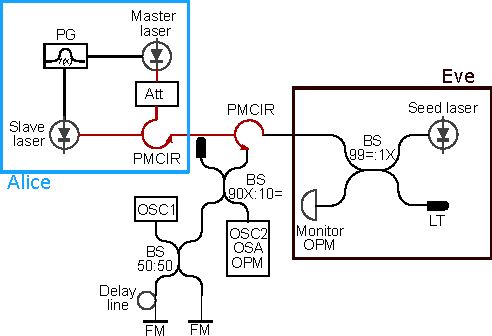
\includegraphics[width=0.9\textwidth]{images/setup_Faraday_Mirrors_final.pdf}
    \caption{Optical schematic diagram of laser source seeding setup based on optical injection}.
    \label{fig:enter-label}
\end{figure}

Two distributed feedback semiconductor lasers were assembled as the source. The first laser was an Agilecom WSLS-934010C4124-42 laser with an integrated isolator, which was used as the master laser to generate the reference radiation. The second laser, however, was an Agilecom WSLS-934010C4124-82 laser, similar to the first laser, but without an integrated insulator. This is to maximize the amount of radiation injected into the resonator of the slave laser. The two lasers are connected to each other via an optical circulator. Its first port is connected to the master laser, the radiation from which enters the second port of the circulator where the slave laser is connected. In this way, the study from the master laser enters the resonator of the slave laser. The radiation from the slave laser enters the second port of the circulator and passes to the third port of the circulator. A Gooch\& Housego AA1406-193300 laser and an erbium fiber amplifier were used as a source of high-power laser radiation. To introduce its radiation, an additional circulator was used, the first port of which was connected to the amplifier output, the second to the third port of the first circulator. A Michelson fiber interferometer was assembled to investigate the interference of the received pulses.
\newline In the course of this work, the characteristics of the output pulses under the influence of external radiation were investigated. The following parameters were studied: amplitude of output pulses and their stability expressed in the measurement of standard deviation, duration of pulses and their standard deviation, as well as the correlation of the phase of the received pulses using a fiber Michelson interferometer. During exposure, the standard deviation of the energy of the output pulses was varied between 2 and 3.5 per cent at an attack laser power of 900 mW and by varying the master laser power. The results of these measurements are shown in Figure \ref{fig:area MDI syn}
\begin{figure}
    \centering
    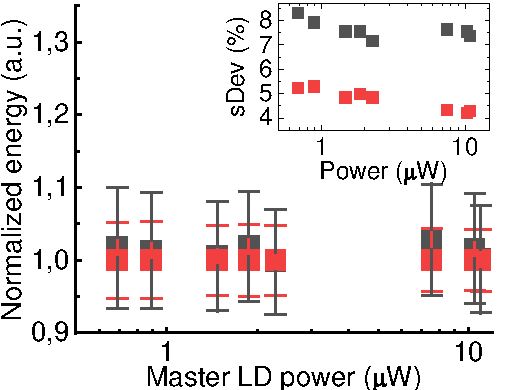
\includegraphics{images/area_under_attack.pdf}
    \caption{Change in source pulse energy with and without external radiation as a function of master laser power}.
    \label{fig:area MDI syn}
\end{figure}
These results show that Eve is able to increase the output power instability to increase the average number of photons per pulse. The pulse duration is also altered by external radiation, shown in Figure \ref{fig:duration syn} the external influence increases the pulse jitter by 2\%.  Existing work shows \cite{xie2019} that even small deviations in pulse duration significantly reduce the distribution range of the secret key. 
\begin{figure}
    \centering
    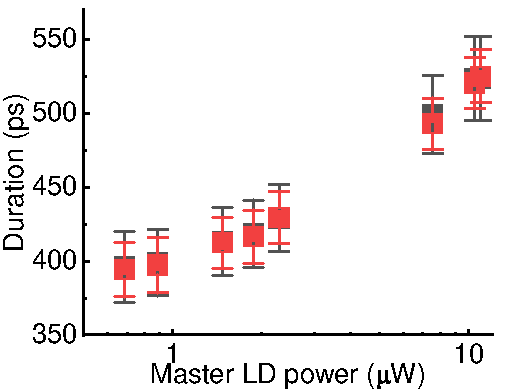
\includegraphics{images/duration_change.pdf}
    \caption{Change in pulse duration due to external radiation}
    \label{fig:duration syn}
\end{figure}
\newline To develop a countermeasure, it is necessary to calculate the necessary isolation factor for the worst case scenario, when the attacker uses the maximum available power. In continuous mode, this value is 2 watts. This value needs to be attenuated to less than -35 dBm. By using a fibre optic circulator as part of the circuit, the isolation value is already 50 dB.  To calculate the required attenuation value, the following formula is used
\begin{equation}
\label{eq:isolation syn}
    \alpha = P_a - P_{req} - \beta.
\end{equation}, where $\alpha$ is the amount of isolation to be introduced, $P_a$ is the amount of probing power in dBm, $P_{req}$ is the power to which the input radiation needs to be attenuated, $\beta$ is the amount of isolation that is already implemented in the circuit, in dB. 
Let's substitute in~\ref{eq:isolation syn} the values of 33 dBm of power, which corresponds to 2 watts of power and 50 dB of isolation. The resulting isolation value required to attenuate 2 watts to -35 dBm is 18 dB. To ensure the safety of this source, it is sufficient to install a fiber isolator with a typical isolation value of 30 dB. This will cover the entire allowable range of sensing power. 
\newline The obtained results demonstrate the resistance of the proposed source of coherent radiation to external influences. To change its characteristics, an intruder needs to operate at powers close to those that trigger a spark in fibre-optic communication lines, which carries an increased risk of being detected. And protocols based on the protocol using an untrusted receiver node are not only secure from attacks of an intruder on receiver nodes in the form of single photon detectors, but also from attacks on single photon sources.
